\chapter{Przegląd istniejących rozwiązań}\label{chap:3_przegląd_istniejących_rozwiązań}

W tym rozdziale przybliżone zostało spektrum dostępnych algorytmów percepcji głębi oraz zbiorów danych używanych do ich trenowania. Zestawienie to ogranicza się do rozwiązań z największą liczbą cytowań w opracowaniach i artykułach naukowych. Osiągają one jednocześnie rekordowe na dzień przygotowywania zestawienia rezultaty.

\section{Algorytmy percepcji głębi}
\subsection{AdelaiDepth}
Zaprojektowany w 2020 r. model AdelaiDepth \cite{yin2020} przygotowany został głównie w celu rekonstrukcji scen trójwymiarowych. Autorzy podzielili wówczas rozwiązanie na dwa etapy - predykcję relatywnej głębi obrazu oraz jej przesunięcie w celu uzyskania głębi metrycznej. Rysunek \ref{fig:adelaidepth} przedstawia wynik działania algorytmu AdelaiDepth.
\begin{figure}[H]
    \centering
    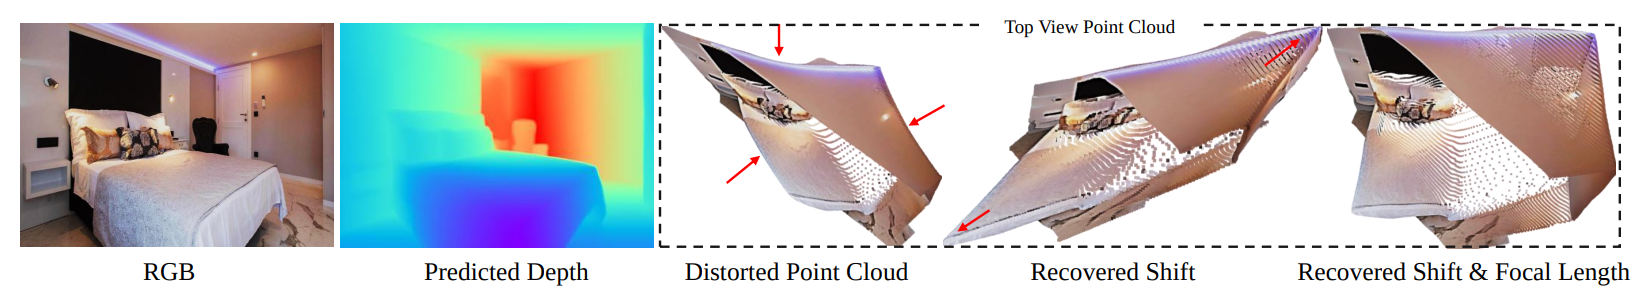
\includegraphics[width=1\textwidth]{8.jpg}
    \caption{Przykładowy wynik działania algorytmu AdelaiDepth. Źródło: \cite{yin2020}}
    \label{fig:adelaidepth}
\end{figure}
Architektura modelu predykcji głębi została zainspirowana rozwiązaniem przedstawionym w \cite{xian2020}. Jest to rekurencyjna sieć neuronowa ResNet \cite{he2015} stanowiąca rodzaj splotowej sieci neuronowej z dekoderem. W celu nauczenia sieci wykorzystano w sumie 354 tysiące obrazów RGBD pochodzących z różnych dostępnych zestawów danych, zarejestrowanych za pomocą urządzeń fizycznych jak i wytworzonych syntetycznie z obrazów RGB za pomocą oprogramowania. Całkowity zestaw danych treningowych zawiera w sobie zatem  wysokiej jakości obrazy z systemu LIDAR ale też niskiej jakości nagrania. Poniższa tabela \ref{fig:adelaidepth-results} obrazuje wyniki osiągane przez ten algorytm na tle wybranych przez autorów podobnych rozwiązań.
\begin{table}[H]
    \centering
    \caption{Porównanie osiąganych wyników przeprowadzone na ośmiu zestawach danych nieuczestniczących w procesie uczenia. Źródło: \cite{yin2020}}
    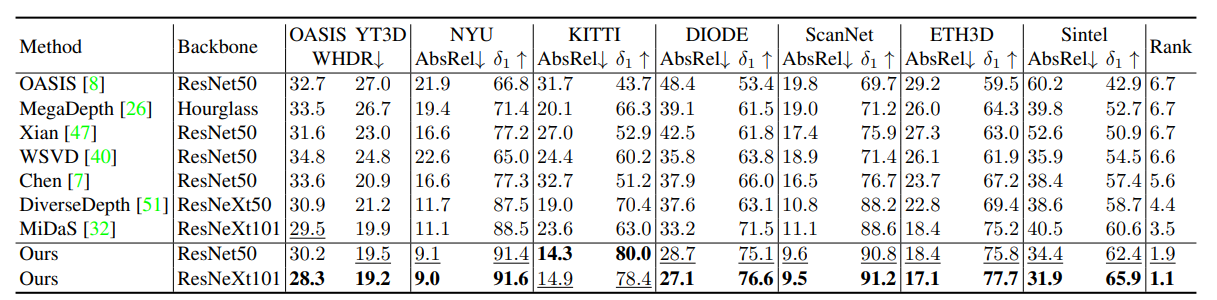
\includegraphics[width=1\textwidth]{9.jpg}
    \label{fig:adelaidepth-results}
\end{table}

\subsection{MetaPrompt-SD}
Głównym założeniem autorów algorytmu MetaPrompt-SD \cite{wan2023} było wykorzystanie modeli dyfuzyjnych w zadaniach dotyczących komputerowej percepcji wizyjnej. Wynikowy model służy do estymacji głębi, segmentacji semantycznej i estymacji pozycji. Przykładowe estymacje przedstawia rys. \ref{fig:metaprompt-sd}.
\begin{figure}[H]
    \centering
    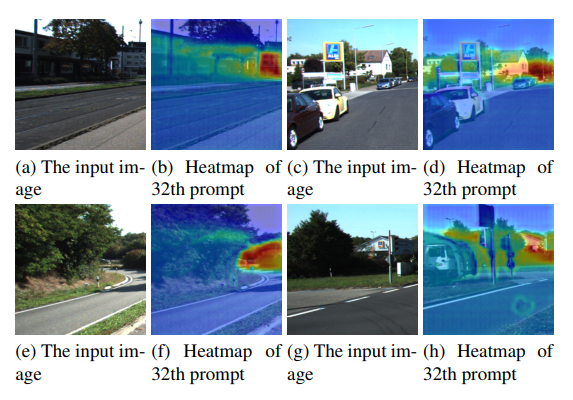
\includegraphics[width=0.6\textwidth]{10.jpg}
    \caption{Przykładowe wyniki działania modułu estymacji głębi MetaPrompt-SD. Źródło: \cite{wan2023}}
    \label{fig:metaprompt-sd}
\end{figure}
Podstawą architektury (rys. \ref{fig:metaprompt-sd-schema}) jest koder VQVAE \cite{oord2018} kodujący obraz wejściowy do przestrzeni ukrytej\footnote{Jest to przestrzeń przechowująca kluczowe cechy obrazu przy jednoczesnej redukcji jego rozdzielczości.} oraz sieć UNet \cite{ronneberger2015}, która wielokrotnie wykorzystana ma za zadanie usunięcie szumów i poprawę jakości cech obrazu. Sieć UNet wspomaga komponent Meta prompts zawierający dodatkowe informacje pomagające w procesie poprawy cech. Po ukończeniu przetwarzania cech obrazu są one wysyłane do dekodera, który przetwarzając je, podaje obraz wyjściowy.
\begin{figure}[H]
    \centering
    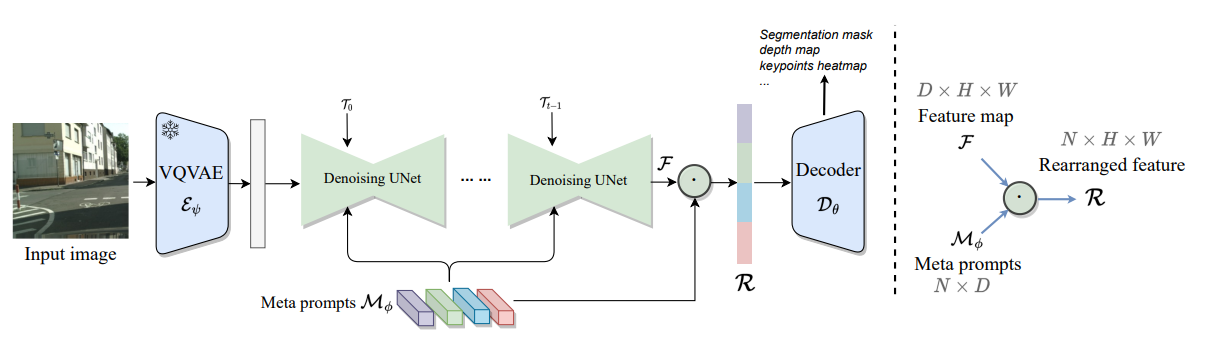
\includegraphics[width=1\textwidth]{11.jpg}
    \caption{Schemat architektury algorytmu MetaPrompt-SD. Źródło: \cite{wan2023}}
    \label{fig:metaprompt-sd-schema}
\end{figure}
Dla percepcji głębi jako zestawy uczące wykorzystane zostały obrazy scen wewnętrznych i zewnętrznych pochodzące ze zbiorów NYU depth V2 oraz KITTI. W sumie stanowi to prawie 95 tysięcy par map głębi z odpowiadającymi im obrazami RGB pochodzącymi z urządzenia LIDAR firmy Velodyne oraz Microsoft Kinect. Tabela \ref{fig:metaprompt-sd-results} zawiera zestawienie wyników w porównaniu z podobnymi rozwiązaniami.
\begin{table}[H]
    \centering
    \caption{Porównanie osiąganych wyników przeprowadzone na dwóch zestawach danych. Źródło: \cite{wan2023}}
    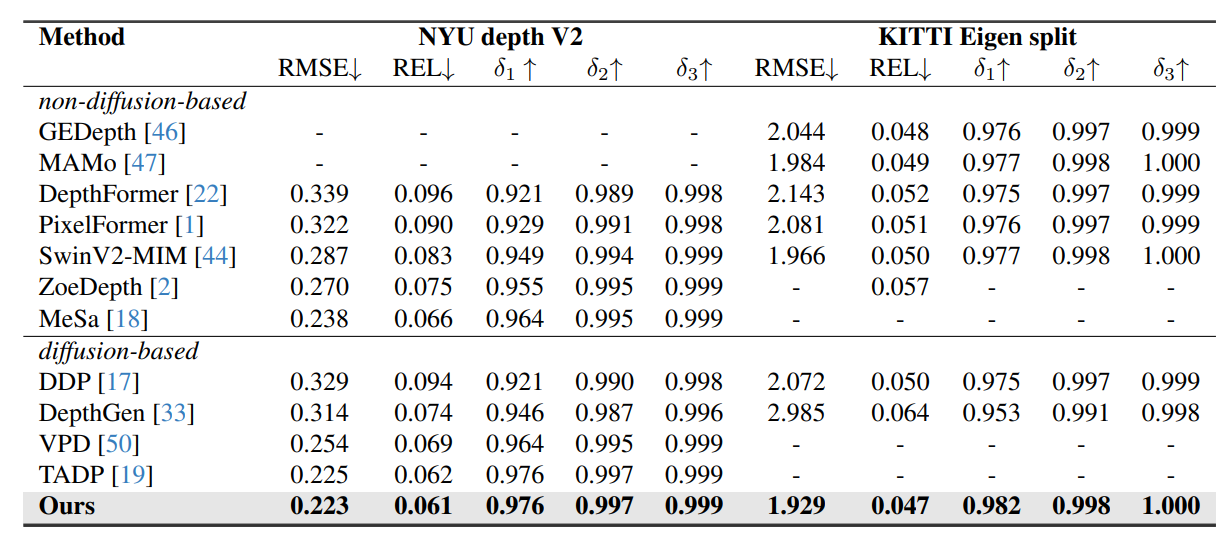
\includegraphics[width=1\textwidth]{12.jpg}
    \label{fig:metaprompt-sd-results}
\end{table}

\subsection{EVP}
Metoda o nazwie EVP \cite{lavreniuk2023} (od ang. Enhanced Visual Perception) jest rozbudowaniem metody VPD \cite{zhao2023} (od ang. Visual Perception with a pre-trained Diffusion model), zadaniem której było podobnie do MetaPrompt-SD wykorzystanie modeli dyfuzyjnych w percepcji wizyjnej. W stosunku do pierwowzoru w modelu EVP dodano moduł o nazwie \textit{IMAFR} (od ang. Inverse MultiAttentive Feature Refinement) wspomagający zdolności wyodrębniania cech. Między innymi dzięki tej zmianie autorom udało się uzyskać lepszy wynik w porównaniu do metody VPD na zestawie NYU Depth v2\footnote{Model EVP uzyskał w tym porównaniu o 11,8\% mniejszą wartość błędu średniokwadratowego.}.
\begin{figure}[H]
    \centering
    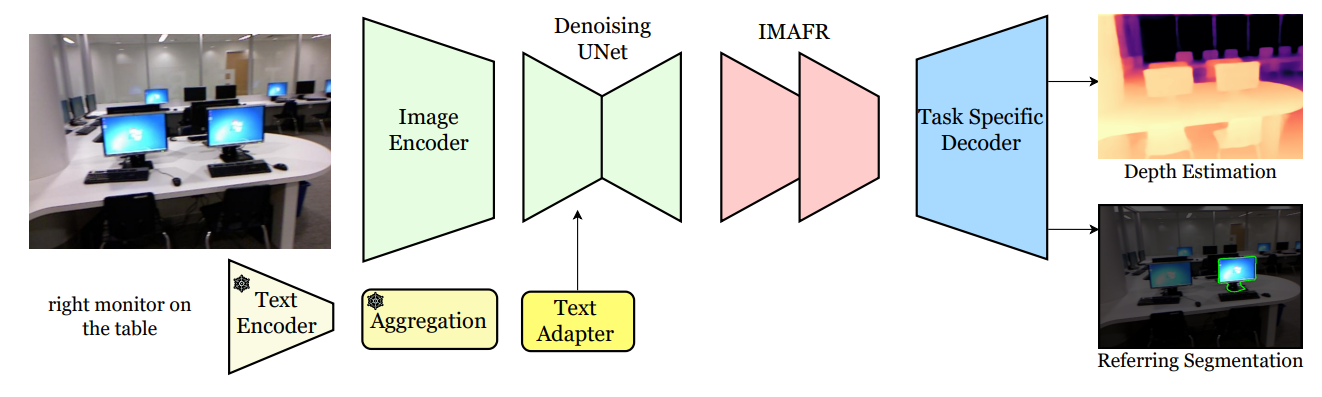
\includegraphics[width=1\textwidth]{13.jpg}
    \caption{Schemat architektury algorytmu EVP. Źródło: \cite{lavreniuk2023}}
    \label{fig:evp-schema}
\end{figure}
Głównymi elementami architektury (rys. \ref{fig:evp-schema}) rozwiązania są koder obrazu wejściowego, sieć wyodrębniająca cechy UNet oraz wyspecjalizowany w kierunku odpowiedniego zadania dekoder. Metoda jest bowiem w stanie wykonać predykcję głębi, jak również dokonać segmentacji semantycznej. Rozwiązanie to zostało wytrenowane przy użyciu zestawów NYU Depth v2 - konkretnie na podzbiorze 50 tysięcy obrazów oraz KITTI - na podzbiorze 26 tysięcy obrazów. Autorzy dokonali porównania rezultatów osiąganych na zbiorze testowym zestawu KITTI - przedstawia je poniższa tabela (rys. \ref{fig:evp-results}).
\begin{table}[H]
    \centering
    \caption{Porównanie osiąganych wyników przeprowadzone na zbiorze KITTI. Źródło: \cite{lavreniuk2023}}
    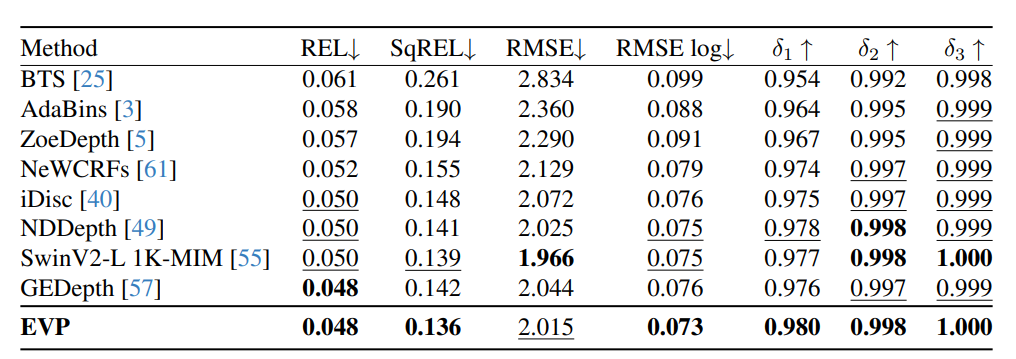
\includegraphics[width=1\textwidth]{14.jpg}
    \label{fig:evp-results}
\end{table}

\subsection{ZoeDepth}
Opracowane rozwiązanie ZoeDepth \cite{bhat2023} skupia się na zachowaniu wydajności przy jednoczesnym użyciu metrycznej skali w wyrażaniu wynikowych predykcji głębi. Proponowany model wykorzystuje 12 różnych zbiorów danych treningowych zawierających głębię relatywną i dwóch zestawów zawierających głębię metryczną, co pozwala osiągnąć założony cel.
\begin{figure}[H]
    \centering
    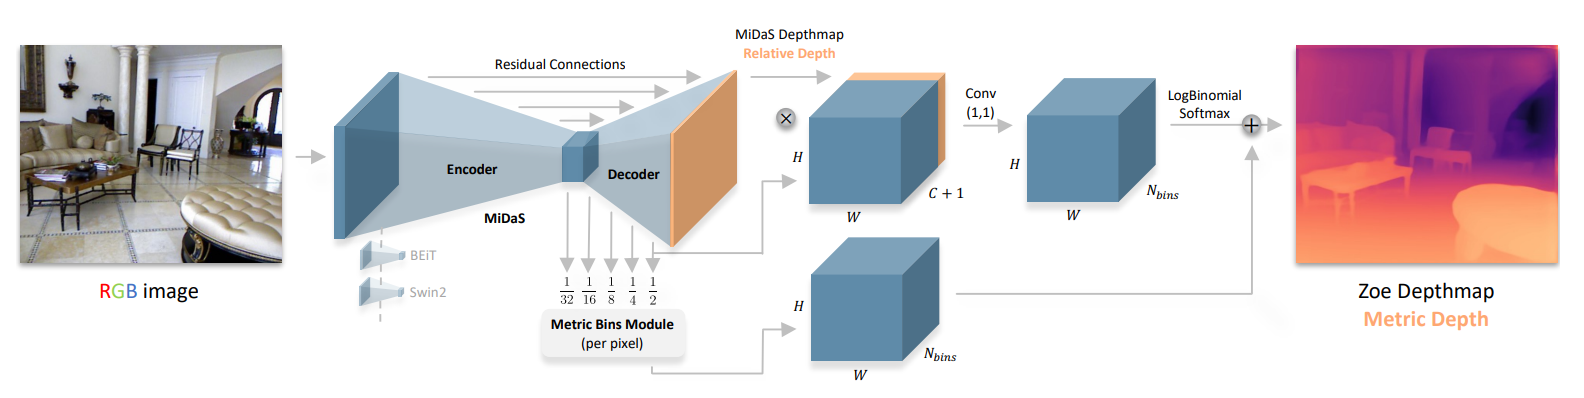
\includegraphics[width=1\textwidth]{15.jpg}
    \caption{Schemat architektury algorytmu ZoeDepth. Źródło: \cite{bhat2023}}
    \label{fig:zoe-schema}
\end{figure}
Architektura algorytmu ZoeDepth (rys. \ref{fig:zoe-schema}) bazuje na rozwiązaniu o nazwie MiDaS \cite{ranftl2020}. Obraz wejściowy jest w pierwszej kolejności przetworzony przez ten właśnie algorytm. Wynik - głębia relatywna - jest dostarczany do modułu metrycznego, którego wynik stanowi z kolei wartość głębi metrycznej dla każdego pojedynczego piksela. Oba te wyniki kierowane są do sieci splotowej i w ten sposób uzyskiwany jest wynik ostateczny - głębia metryczna. Istnieje pięć gotowych przetrenowanych modeli, nazwanych według szablonu ZoeD-[zestaw pierwszy]-[zestaw drugi], gdzie zestawem pierwszym jest zestaw treningowy obrazów z głębią relatywną, a zestaw drugi zawiera obrazy z głębią metryczną. Litera "X" w miejscu zestawu pierwszego oznacza, że w celu uczenia modelu wykorzystany został jedynie zestaw drugi. Tabela \ref{fig:zoe-results} zawiera porównanie wyników na zestawie NYU-Depth v2.
\begin{table}[H]
    \centering
    \caption{Porównanie osiąganych wyników przeprowadzone na zbiorze NYU-Depth v2. Źródło: \cite{bhat2023}}
    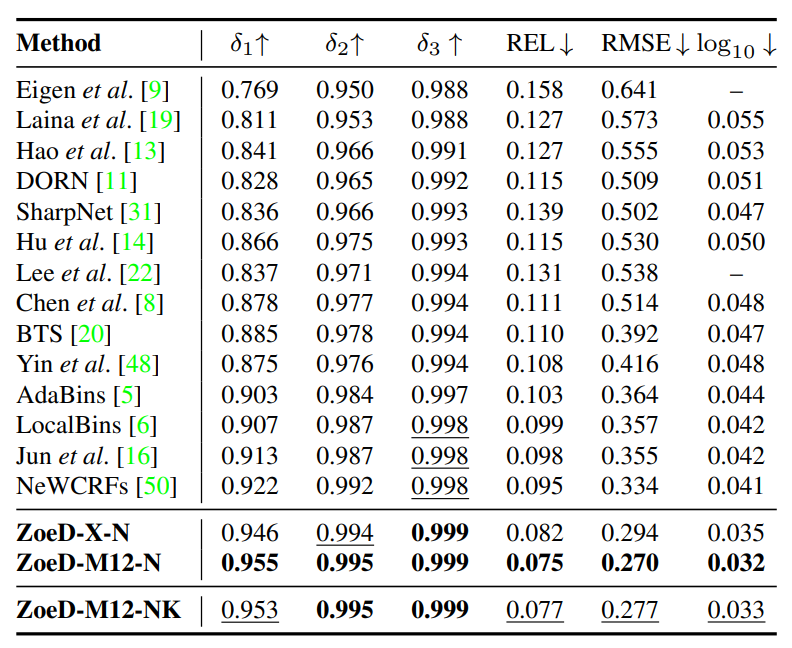
\includegraphics[width=0.60\textwidth]{16.jpg}
    \label{fig:zoe-results}
\end{table}

\subsection{UniDepth}
Model o nazwie UniDepth \cite{piccinelli2024} został zaproponowany przez jego autorów naprzeciw ich tezie o niskim stopniu generalizacji konkurencyjnych modeli. W swojej publikacji twierdzą, że ówcześnie najlepsze pod względem osiąganych wyników modele do predykcji głębi weryfikowane są na zbiorach podobnych do uczących oraz często na tyle niewielkich, że wyniki osiągane na pojedynczych obrazach odbiegających od domeny zbiorów uczących są mniej zadowalające.
Architektura sieci tego modelu (rys. \ref{fig:unidepth-schema}) składa się z trzech głównych modułów - kodera, kamery i głębi. Koder przetwarza obraz wejściowy do postaci cech, które następnie przesyłane są do kolejnych dwóch modułów. Może być zarówno oparty o sieć splotową jak i o transformator wizyjny ViT co ma pozwolić na elastyczne dopasowanie do potrzeb użytkownika. Moduł kamery odpowiada za generowanie reprezentacji, która jest następnie wykorzystywana do warunkowania cech głębi. Moduł głębi przyjmuje cechy z kodera i warunkuje je na podstawie informacji z modułu kamery, wykorzystując przy tym warstwę uwagi krzyżowej. Połączenie wyniku modułu kamery i modułu głębi to wynik działania całego algorytmu.
\begin{figure}[H]
    \centering
    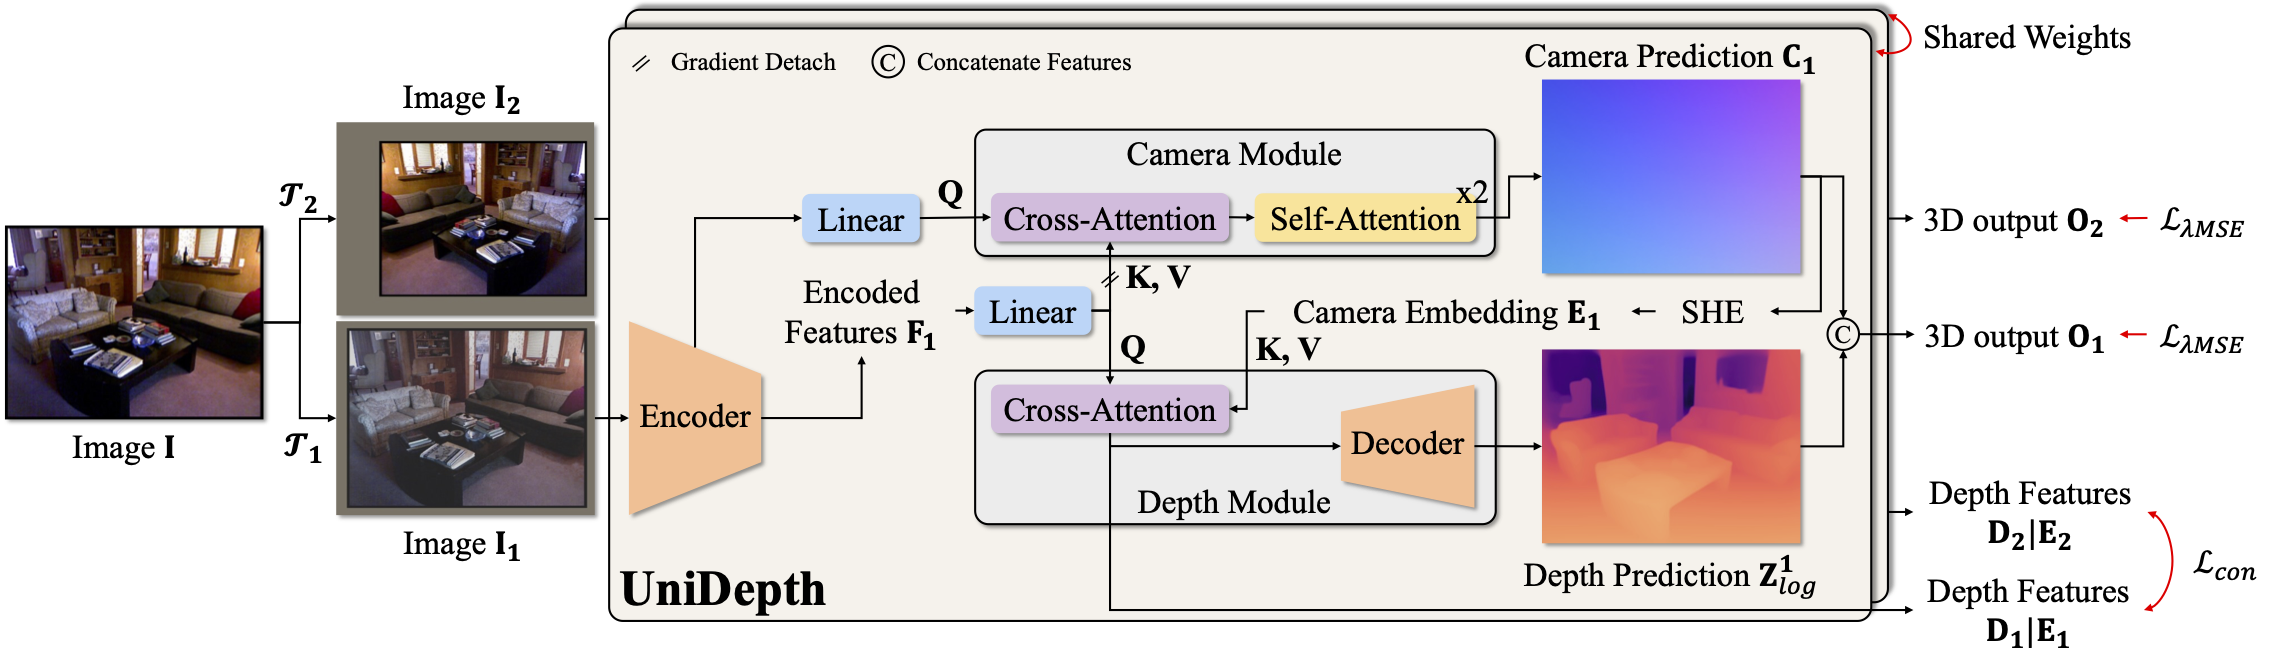
\includegraphics[width=1\textwidth]{21.jpg}
    \caption{Schemat architektury algorytmu UniDepth. Źródło: \cite{piccinelli2024}}
    \label{fig:unidepth-schema}
\end{figure}
Do nauczenia modelu UniDepth wykorzystano 9 zestawów uczących składających się łącznie na 3 miliony obrazów, co umożliwiło nauczenie modelu rożnorodnych scen z różnych punktów widzenia i różnymi warunkami oświetleniowymi. Do weryfikacji rezultatów wykorzystano natomiast 10 zestawów danych niepokrywających się z zestawami uczącymi. W porównaniu rezultatów wykorzystano modele zawierające koder z transformatorem i z siecią splotową, odpowiednio UniDepth-V i UniDepth-C. Tabela \ref{fig:unidepth-results} przedstawia porównanie rezultatów modelu UniDepth.
\begin{table}[H]
    \centering
    \caption{Porównanie rezultatów UniDepth dokonane na zbiorach danych niewidzianych podczas uczenia. Źródło: \cite{piccinelli2024}}
    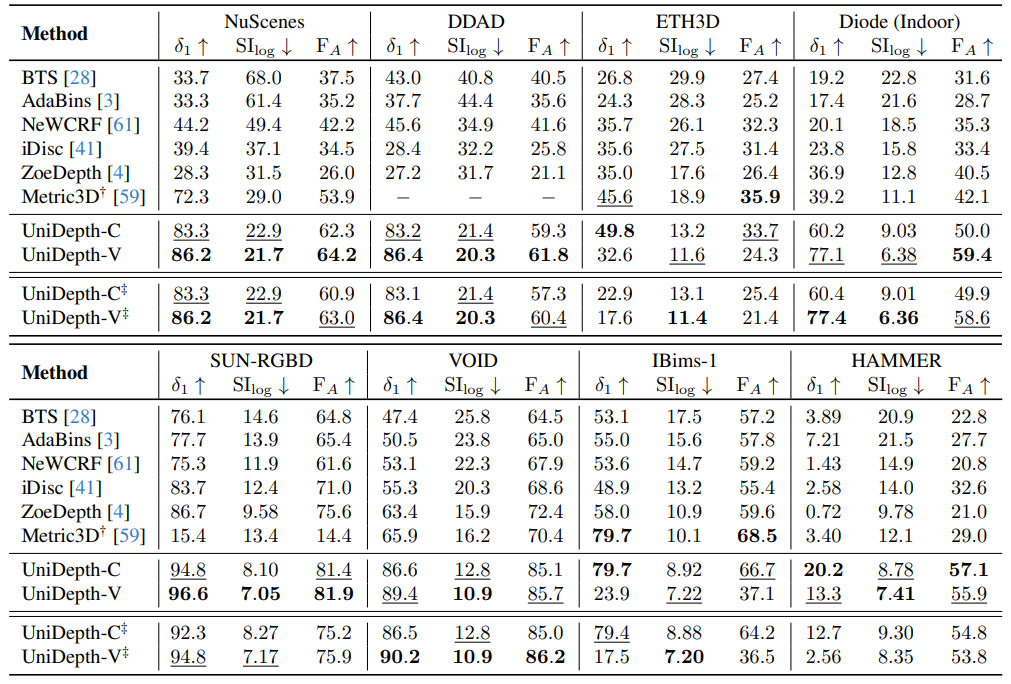
\includegraphics[width=0.95\textwidth]{22.jpg}
    \label{fig:unidepth-results}
\end{table}

\subsection{Depth Anything V2}
Interesującą strategię rozwiązania przyjęli autorzy modelu Depth Anything V2 \cite{yang2024depth}. Położyli oni bowiem nacisk na niezwykle duży zestaw danych uczących składający się nie tylko z danych oznaczonych (595 tysiące obrazów), ale również z danych nieoznaczonych (62 miliony obrazów). Wykorzystane zbiory danych przedstawione są w tabeli \ref{fig:depth-anything-data}. Jest to w związku z tym model uczony metodą częściowo nadzorowaną. W ten sposób otrzymano model charakteryzujący się bardzo dużą zdolnością generalizacji na nowych scenach. W stosunku do pierweszej wersji modelu \cite{yang2024depthv1} poprawiono wydajność, poprawność estymacji na odbiciach i obiektach przezroczystych oraz zastosowano uczenie na bardziej skomplikowanych scenach. Jako priorytet twórcy ustanowili estymację głębi relatywnej, dopiero po dostrojeniu modelu z użyciem zestawu KITTI lub NYUv2 model ten zyskuje zdolność predykcji głębi metrycznej. Poniżej znajduje się rysunek \ref{fig:depth-anything} z porównaniem z wersją pierwszą oraz konkurencyjnym modelem.
\begin{figure}[H]
    \centering
    \includegraphics[width=0.85\textwidth]{17.jpg}
    \caption{Depth Anything V2 w porównaniu z wersją pierwszą i modelem Marigold \cite{ke2024repurposing}. Źródło: \cite{yang2024depth}}
    \label{fig:depth-anything}
\end{figure}
W architekturze tego rozwiązania (rys. \ref{fig:depth-anything-schema}) zastosowano koder wyodrębniający cechy obrazu wejściowego przygotowany na podstawie DINOv2 \cite{oquab2024} oraz dekoder DPT do regresji głębi. W pierwszej kolejności model "nauczyciela" uczony jest na zestawie danych oznaczonych. Następnie model ten wykorzystywany jest w celu oznaczenia zbioru danych nieoznaczonych, który razem z zestawem danych oznaczonych weźmie udział w procesie uczenia modelu "ucznia".
\begin{figure}[H]
    \centering
    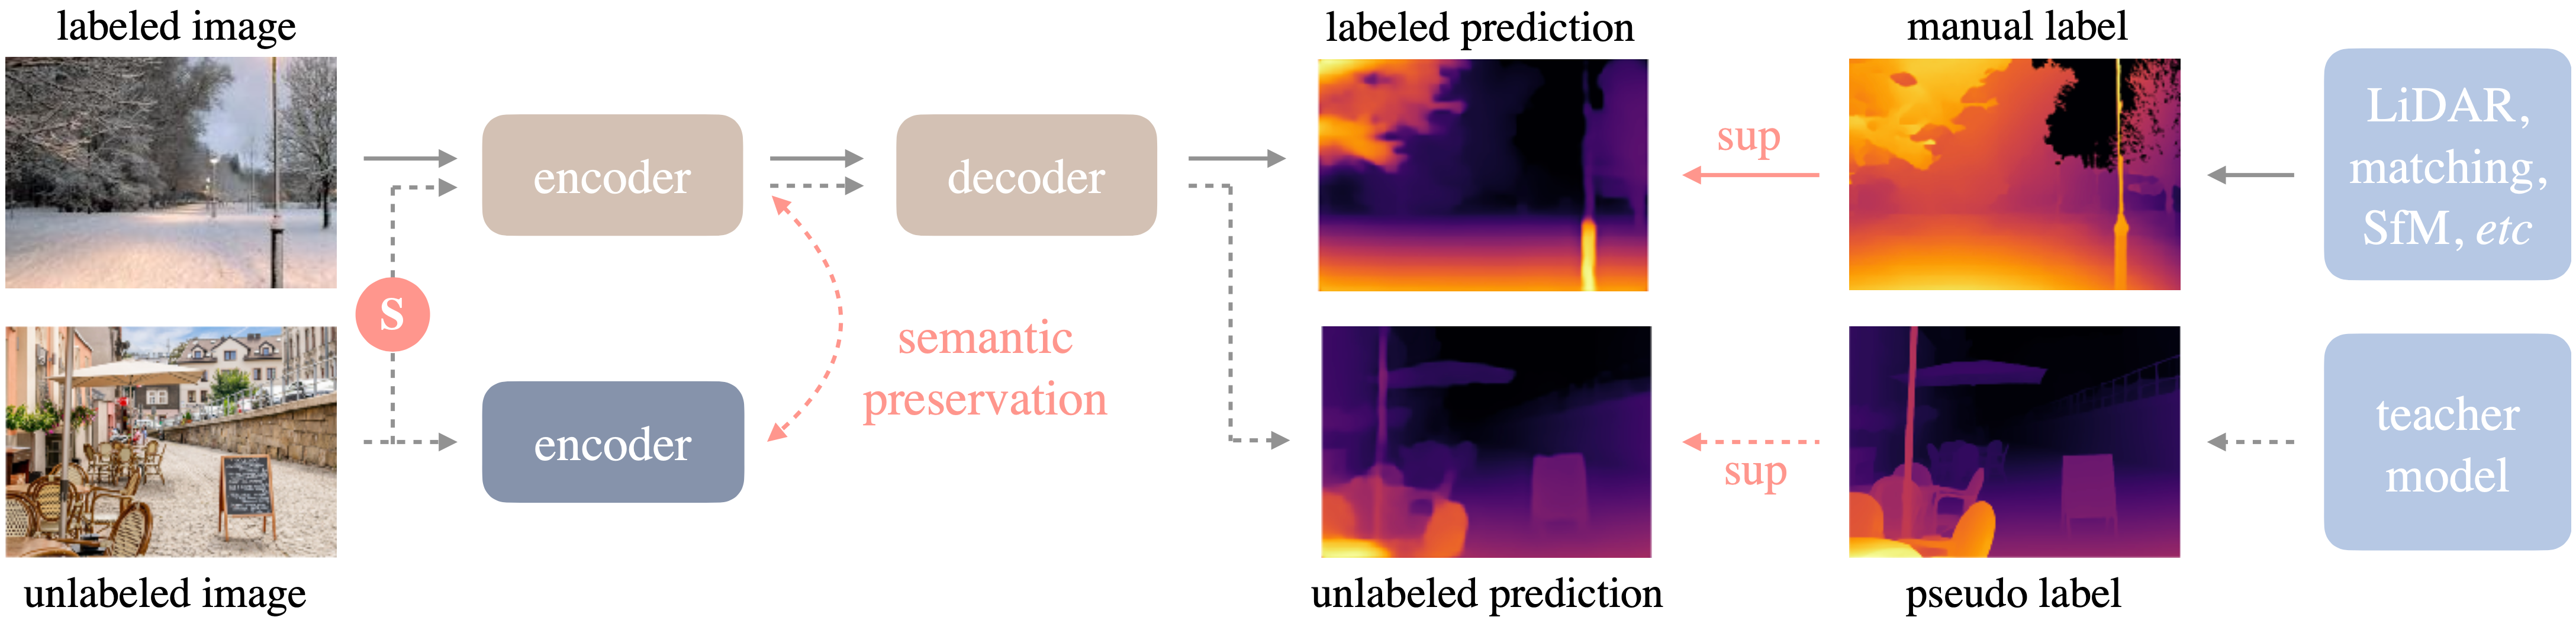
\includegraphics[width=0.9\textwidth]{18.jpg}
    \caption{Schemat architektury algorytmu Depth Anything. Źródło: \cite{yang2024depth}}
    \label{fig:depth-anything-schema}
\end{figure}
\begin{table}[H]
    \centering
    \caption{Zbiór zestawów danych uczących Depth Anything. Źródło: \cite{yang2024depth}}
    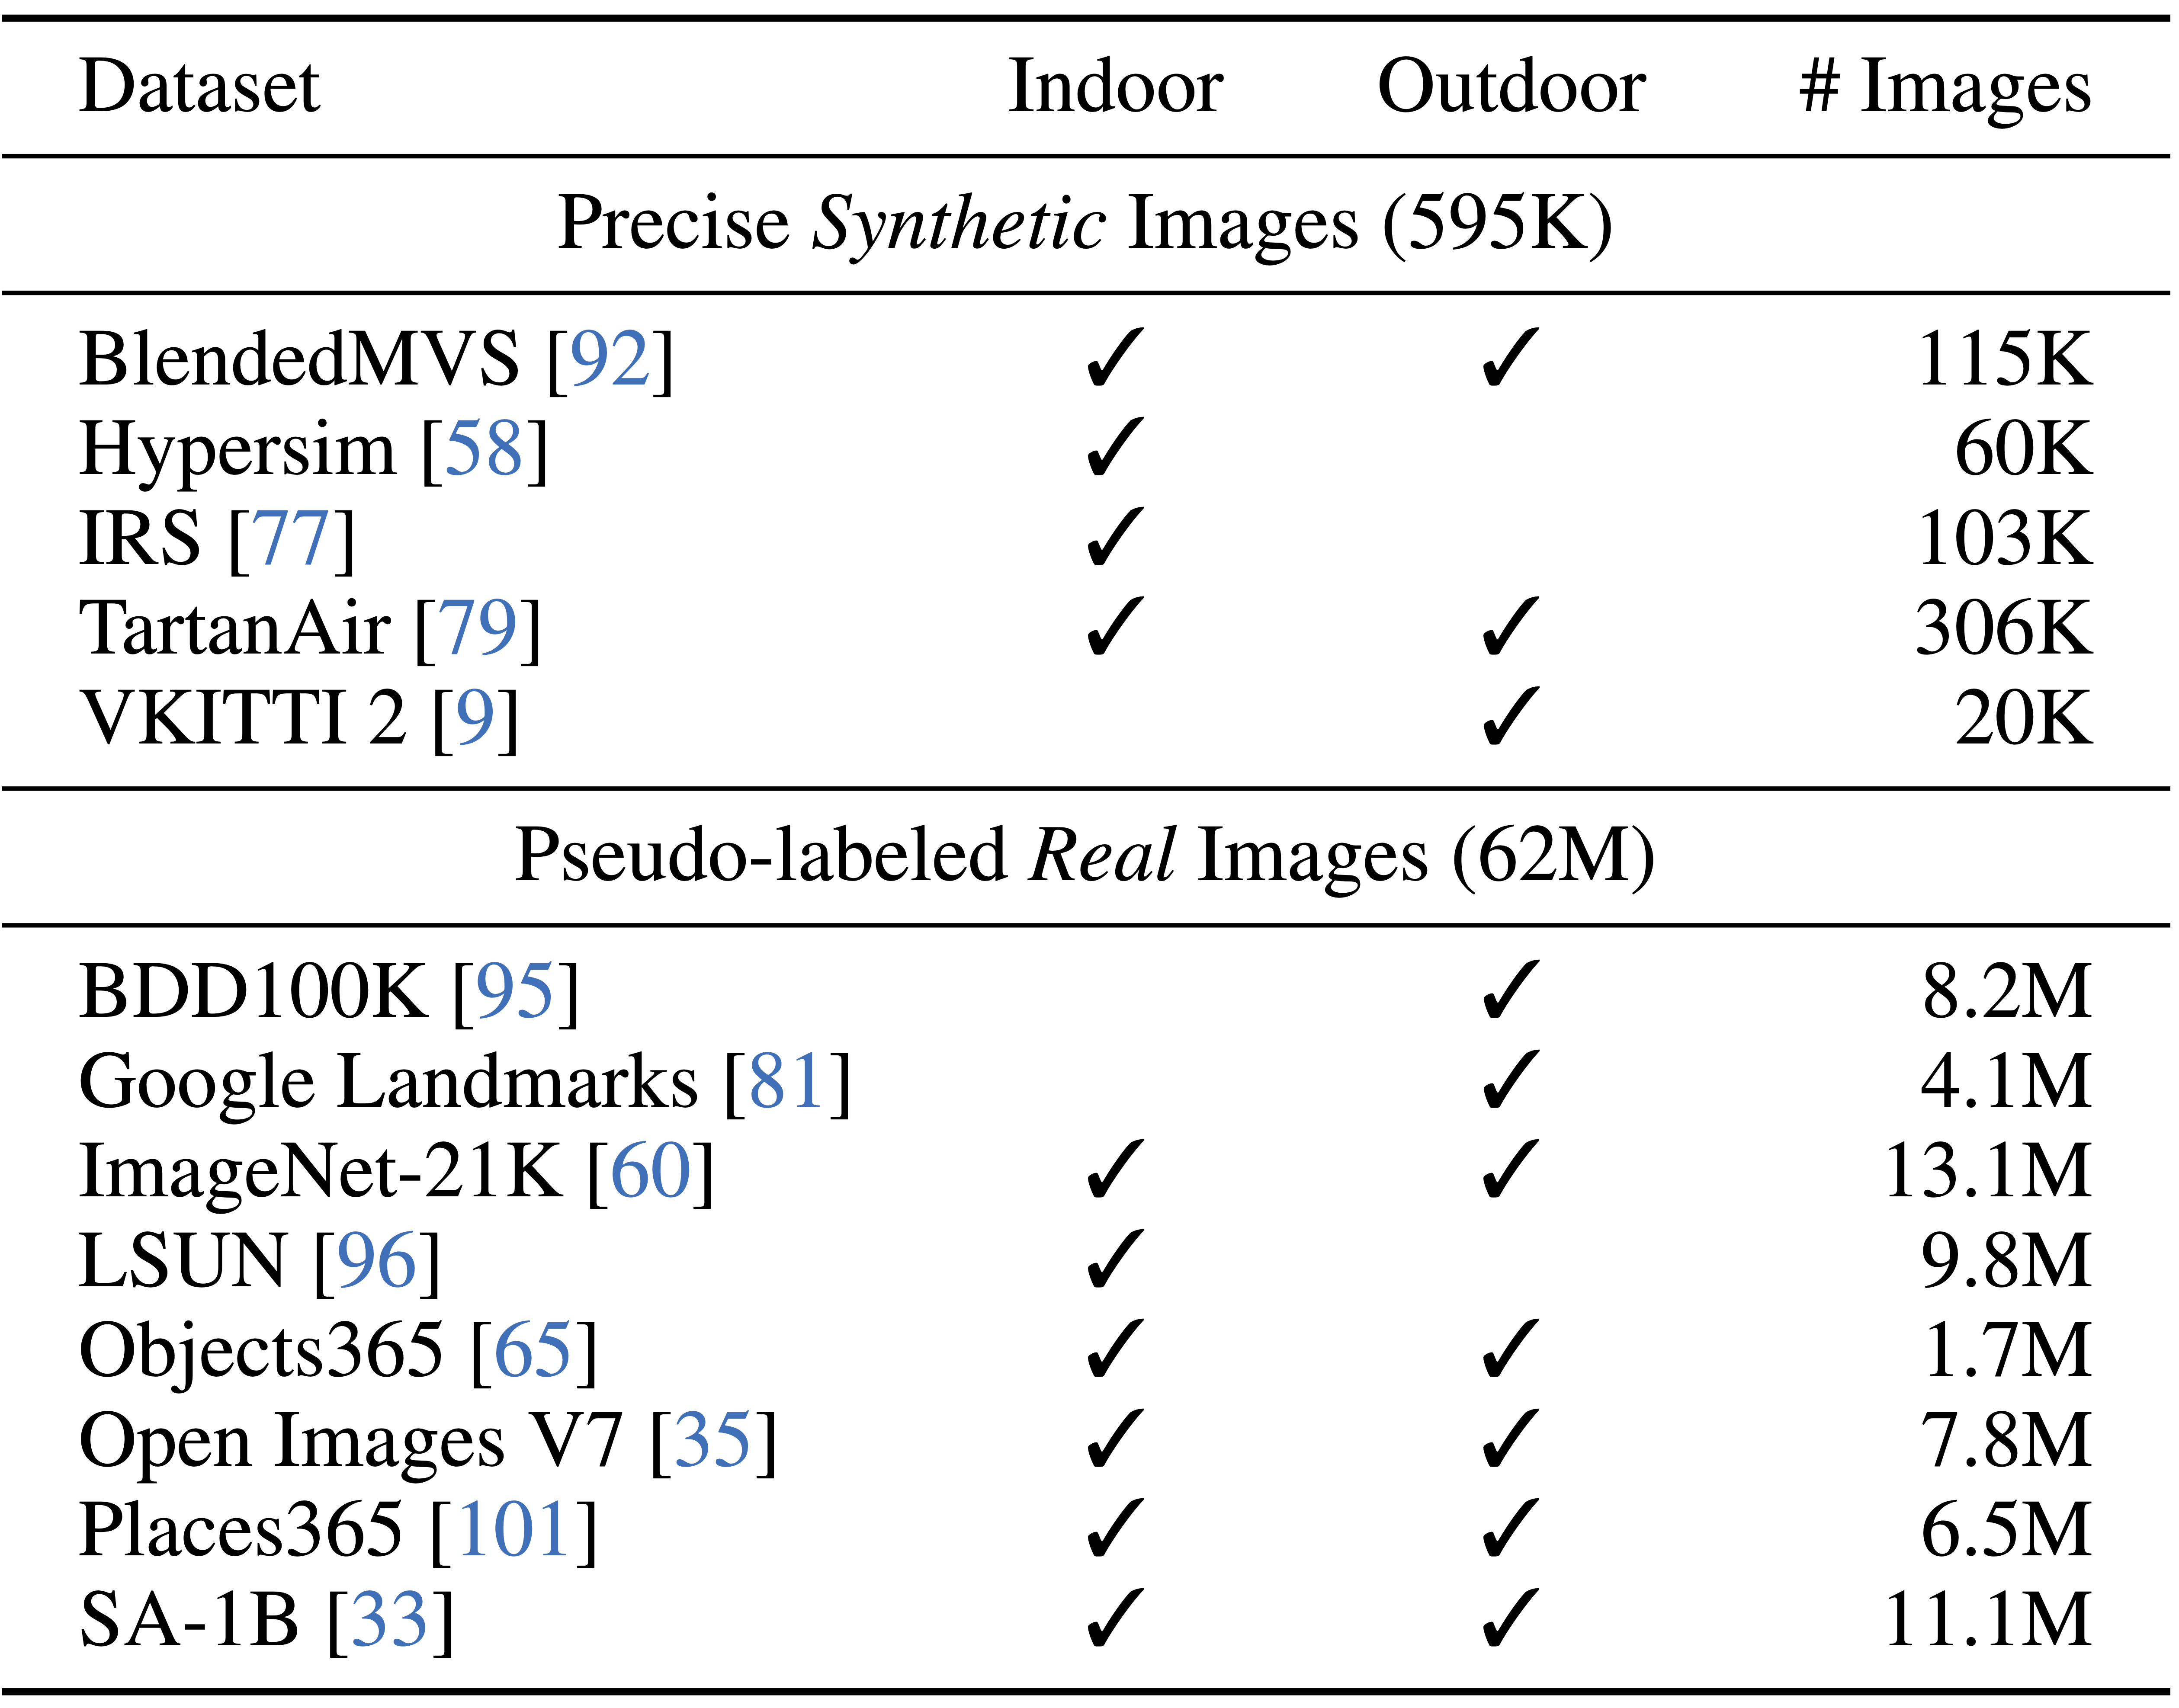
\includegraphics[width=0.6\textwidth]{19.jpg}
    \label{fig:depth-anything-data}
\end{table}
Osiągane wyniki w porównaniach przeprowadzonych na zbiorach danych testowych (tabela \ref{fig:depth-anything-results}) w sposób zdecydowany udowadniają tezę autorów dotyczącą zasadności skalowania zestawów uczących przy pomocy danych nieoznaczonych.
\begin{table}[H]
    \centering
    \caption{Porównanie rezultatów Depth Anything dokonane na podstawie zbioru NYUv2 (po lewej) i KITTI (po prawej). Źródło: \cite{yang2024depth}}
    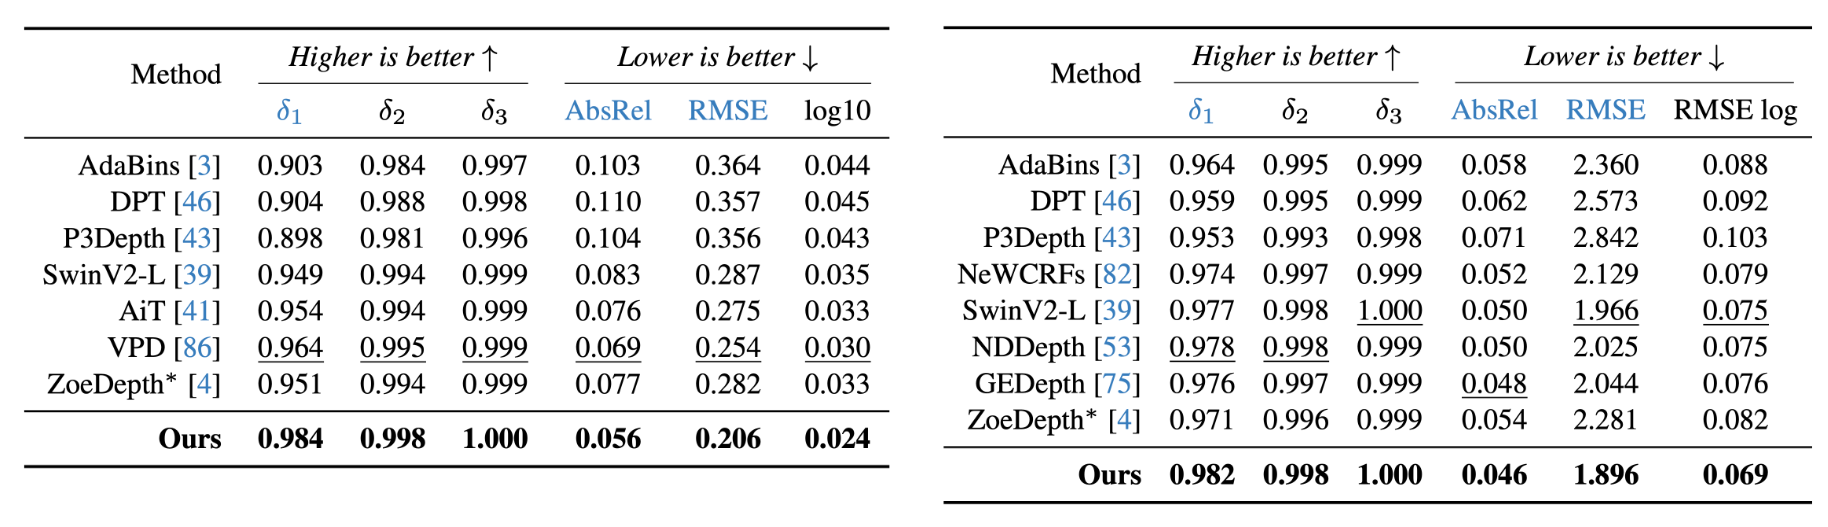
\includegraphics[width=1\textwidth]{20.jpg}
    \label{fig:depth-anything-results}
\end{table}

\subsection{Metric3D V2}
Metoda Metric3D V2 \cite{hu2024} adresuje dwa kluczowe problemy: estymację metrycznej głębokości i normalnych powierzchni z pojedynczego obrazu. Jest ona zaprojektowana z uwzględnieniem wysokiej generalizacji, w związku z czym bez dodatkowego dostrajania można ją wykorzystać w celu predykcji na obrazach prezentujących zróżnicowane sceny.
Głębokość metryczna pozwala na precyzyjne odwzorowanie rzeczywistego świata, podczas gdy normalne powierzchni zapewniają szczegółową geometrię lokalną. Ostateczny wynik powstaje dzięki dostosowaniu wyniku estymacji za pomocą danych dotyczących matrycy aparatu rejestrującego. 

Do trenowania modelu użyto dużego zestawu danych obejmującego 18 różnych zbiorów, które łącznie zawierają ponad 16 milionów obrazów. Zbiory te pochodzą z różnych typów scen, zarówno wewnętrznych jak i zewnętrznych, oraz obejmują różne modele kamer. Do testowania natomiast użyto zestawów danych 7 zestawów częściowo pokrywających się z zestawami uczącymi.

\begin{figure}[H]
    \centering
    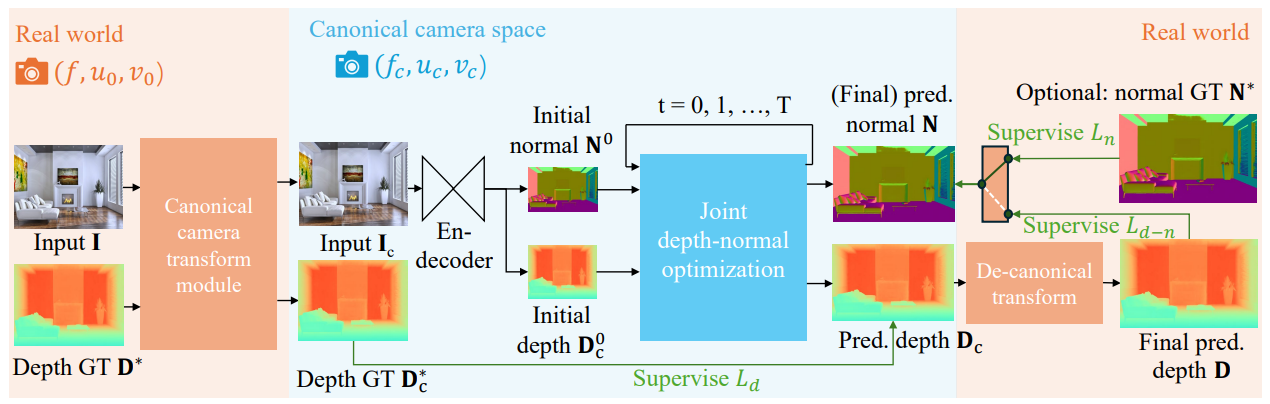
\includegraphics[width=1\textwidth]{25.jpg}
    \caption{Uproszczony schemat architektury rozwiązania Metric3D. Źródło: \cite{hu2024}}
    \label{fig:metric3d-schema}
\end{figure}

Autorzy tej metody zastosowali w niej zarówno architekturę opartą o splotową sieć neuronową (UNet), jak i transformator (ViT i DPT jako dekoder), w zależności od konfiguracji metoda może korzystać z jednej z nich. Uproszczony schemat architektury widnieje na rys. \ref{fig:metric3d-schema}. Wyniki Metric3D na dzień opracowania bieżącego rozdziału ustanawiają nowy stan sztuki osiąganymi wynikami, które prezentuje poniższa tabela \ref{fig:metric3d-results}.
\begin{table}[H]
    \centering
    \caption{Porównanie rezultatów Metric3D do innych wiodących metod. Źródło: \cite{hu2024}}
    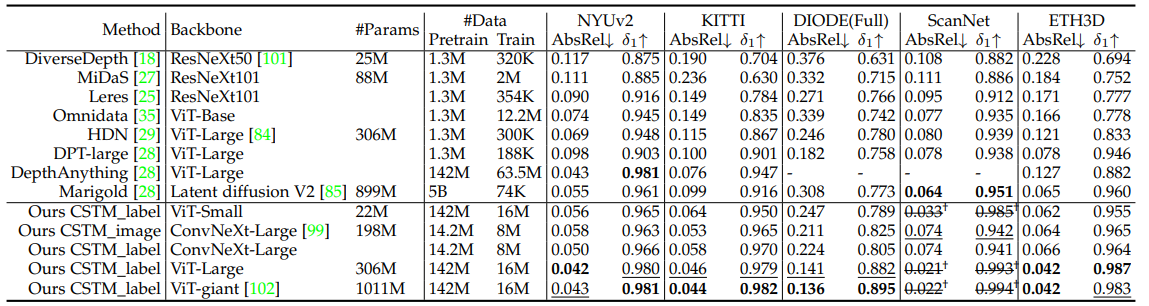
\includegraphics[width=1\textwidth]{26.jpg}
    \label{fig:metric3d-results}
\end{table}

\subsection{DistDepth}
Autorzy pracy prezentującej metodę DistDepth \cite{wu2022practical} zwracają uwagę na to, że dostępne obecnie metody skupiające się na obrazach przedstawiających ruch uliczny, nie znajdują dobrego zastosowania w predykcji głebi na obrazach przedstawiających skomplikowane sceny wewnętrzne, szczególnie takie, które na planie posiadają wiele gęsto ulokowanych przedmiotów. Proponują oni rozwiązanie składające się z dwóch części - estymatora struktur ze względnymi wartościami głębokości opartego o transformator wizyjny, którego wynik wraz z obrazem wejściowym wysyłany jest na wejście estymatora głębi opartego o splotową sieć neuronową trenowanego w sposób nienadzorowany. W ten sposób uzyskany model w czasie rzeczywistym wnioskuje głębię pojedynczego obrazu z wysoką generalizacją pośród scen wewnętrznych. Schemat działania algorytmy DistDepth zaprezentowano na rys. \ref{fig:distdepth-teaser}.
\begin{figure}[H]
    \centering
    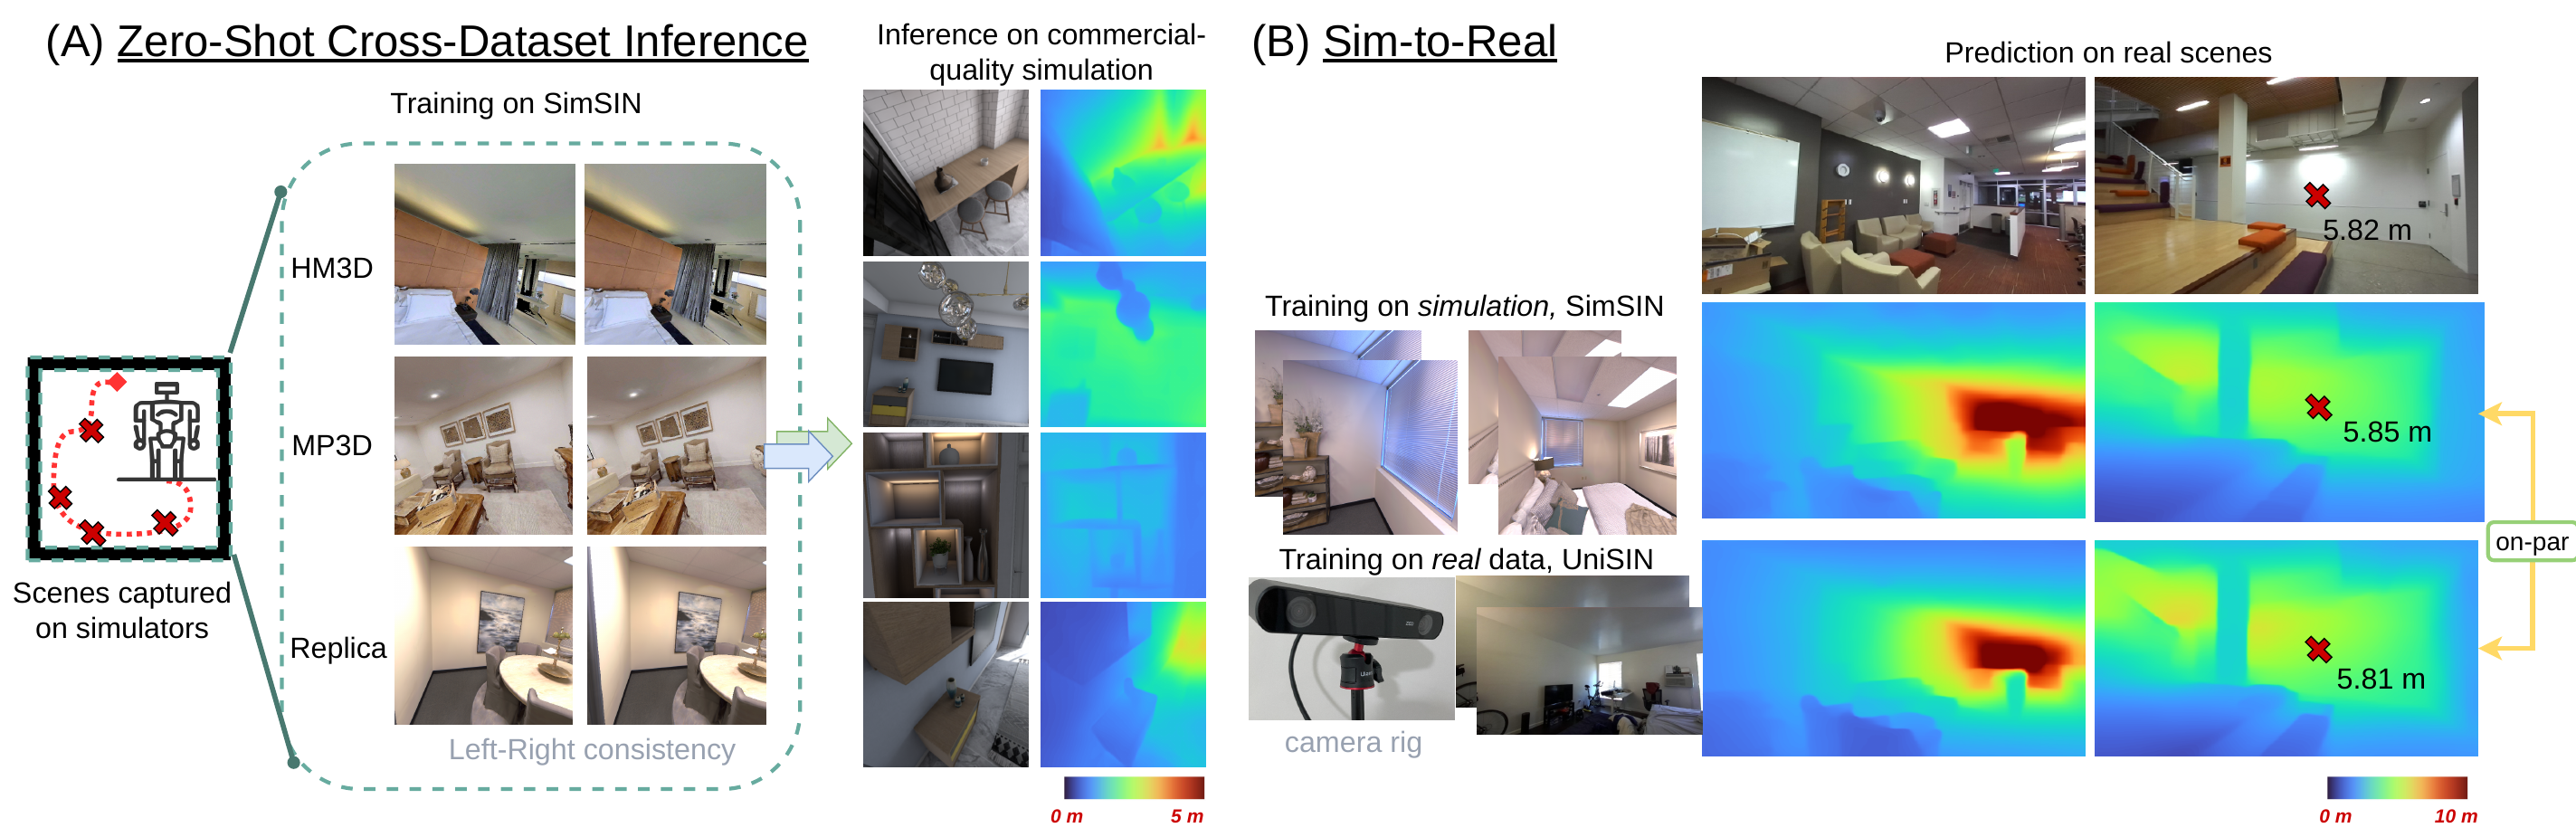
\includegraphics[width=1\textwidth]{27.jpg}
    \caption{Schemat przedstawiający działanie algorytmu DistDepth. Źródło: \cite{wu2022practical}}
    \label{fig:distdepth-teaser}
\end{figure}
W celu nauczenia algorytmu DistDepth wykorzystano dwa autorskie zestawy danych - SimSIN zawierający 500 tysięcy symulowanych komputerowo obrazów scen wewnętrznych w postaci par stereo (ponieważ uczenie odbywa się w sposób nienadzorowany, sceny nie zawierają żadnej informacji o głębi) oraz UniSIN zawierający 200 tysięcy obrazów scen przedstawiających wnętrza uniwersytetu zarejestrowanych za pomocą urządzenia ZED 2I \cite{ZED2I}. Wyniki osiągane przez model DistDepth przedstawia tabela \ref{fig:distdepth-results}.
\begin{table}[H]
    \centering
    \caption{Porównanie wyników z innymi rozwiązaniami wykonane na zestawie NYU v2. Źródło: \cite{wu2022practical}}
    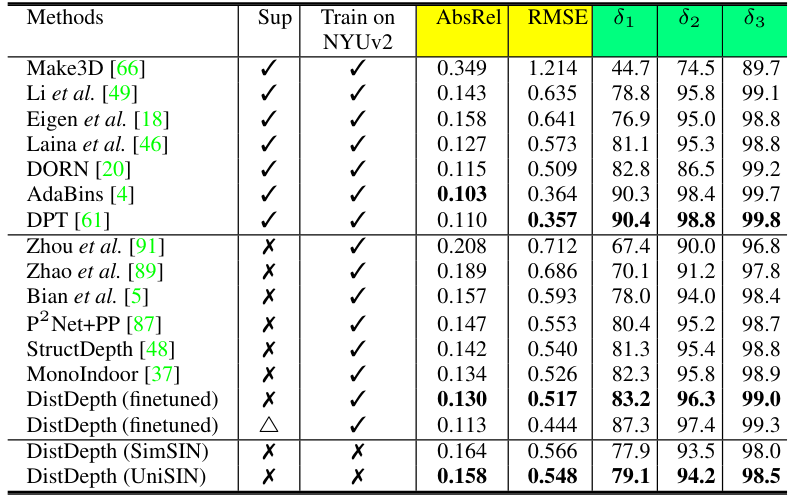
\includegraphics[width=0.75\textwidth]{28.jpg}
    \label{fig:distdepth-results}
\end{table}

\subsection{GCNDepth}
Wykorzystujący architekturę grafowej splotowej sieci neuronowej \cite{GNNBook2022} model GCNDepth \cite{masoumian2021gcndepth} oferuje według twórców 89\% skuteczność na publicznie dostępnych zbiorach KITTI i Make3D, redukując jednocześnie o 40\% ilość trenowanych parametrów sieci w porównaniu z innymi obecnymi algorytmami. Model ten koncentruje się na scenach plenerowych, szczegónie na ruchu ulicznym ze względu na charakterystykę obrazów trenujących. Precyzując, architektura (rys. \ref{fig:gcn-schema}) składa się z dwóch głównych komponentów: sieci DepthNet odpowiedzialnej za przewidywanie map głębokości oraz sieci PoseNet odpowiedzialnej za przewidywanie pozy aparatu między kolejnymi klatkami wideo ze względu na nienadzorowane uczenie algorytmu. Poniższy rysunek \ref{fig:gcn-schema} zawiera schemat opisanej architektury.
\begin{figure}[H]
    \centering
    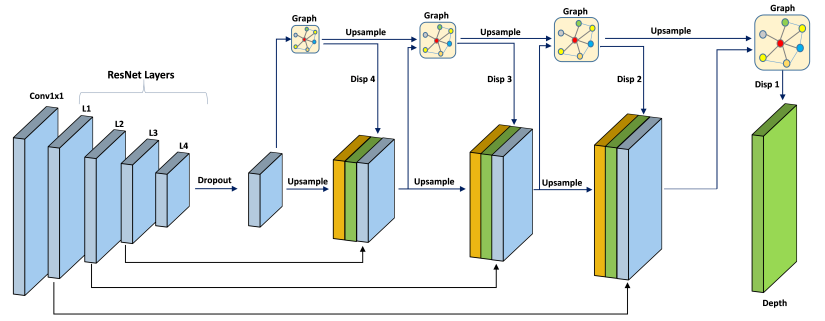
\includegraphics[width=0.75\textwidth]{29.jpg}
    \caption{Schemat przedstawiający architekturę modelu GCNDepth. Źródło: \cite{GNNBook2022}}
    \label{fig:gcn-schema}
\end{figure}
Zbiór trenujący modelu GCNDepth stanowi 200 nagrań wideo ruchu ulicznego w świetle dziennym z publicznego zestawu KITTI. Na tym zestawie oraz na Make3D autorzy dokonali testów uzyskanego modelu. Wyniki w porównaniu do podobnych rozwiązań przedstawione zostały w postaci tabeli \ref{fig:gcn-results}.
\begin{table}[H]
    \centering
    \caption{Wyniki GCNDepth uzyskane na zestawie KITTI w porównaniu z podobnymi rozwiązaniami. Źródło: \cite{GNNBook2022}}
    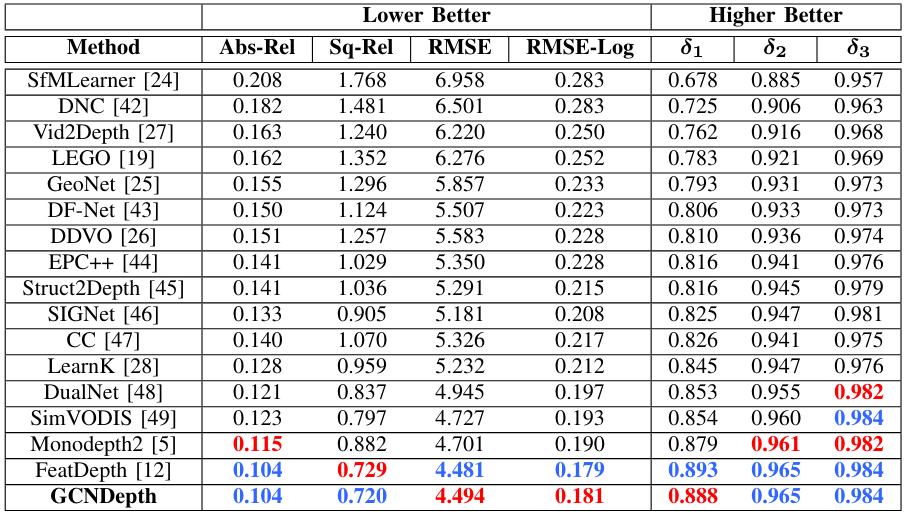
\includegraphics[width=0.75\textwidth]{30.jpg}
    \label{fig:gcn-results}
\end{table}


\subsection{M4Depth}
Metoda M4Depth \cite{fonder2023technique} została zaprojektowana z myślą o bezzałogowych statkach powietrznych. Jej autorzy podkreślają, jak istotne jest oszacowanie niepewności obok estymacji głębokości w tym konkretnym zastosowaniu. Ponadto w tak niewielkich statkach powietrznych waga stanowi kwestię kluczową, przez co jeden obiektyw zamiast dwóch jest zdecydowanie lepszym wyborem. Metoda ta ma być według autorów ponad 2 razy szybsza przy zachowaniu podobnej dokładności, co również nie pozostaje obojętne w kontekście lotów dronem. Architektura rozwiązania to piramidowa splotowa sieć neuronowa na wzór PWC-Net \cite{sun2018pwcnet}. Rysunek \ref{fig:m4d-schema} zawiera schemat działania modelu M4Depth.
\begin{figure}[H]
    \centering
    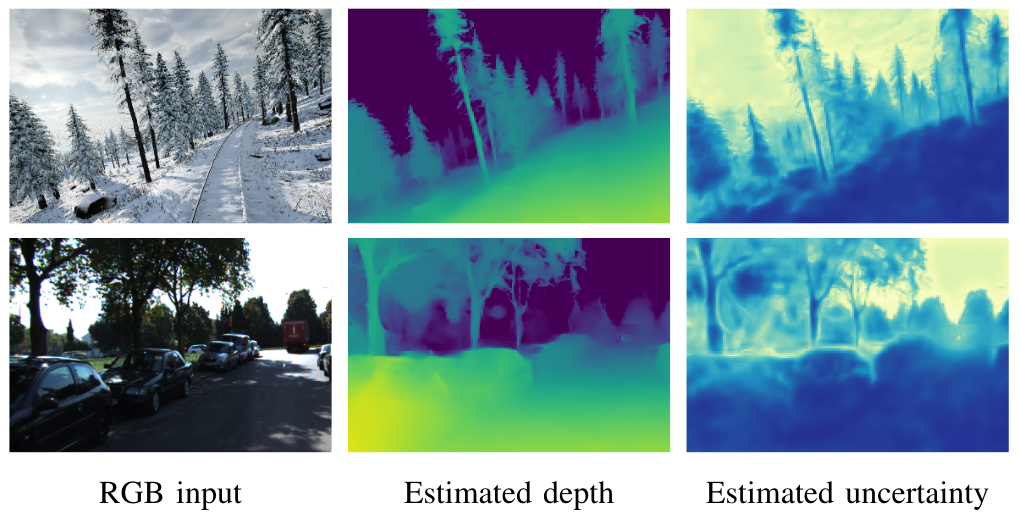
\includegraphics[width=0.6\textwidth]{31.jpg}
    \caption{Schemat działania modelu M4Depth. Źródło: \cite{fonder2023technique}}
    \label{fig:m4d-schema}
\end{figure}
W zależności od zastosowanej funkcji straty - jednej z dwóch - wykorzystanej w procesie uczenia model przyjmuje nazwę M4Depth+U\textsubscript{$\rho$} lub M4Depth+U\textsubscript{z}.
Model został wytrenowany na zbiorze Mid-Air \cite{fonder2019midair}, czyli syntetycznych obrazach stanowiących wizualizacje lotu dronem zawierających między innymi informację o głębi sceny. Testy dokonano natomiast przy użyciu zbiorów Mid-Air, KITTI oraz TartanAir \cite{wang2020tartanair}. Tabela \ref{fig:m4d-comparison} zawiera porównanie z innymi modelami, należy zwrócić uwagę na czas wymagany na estymację przez poszczególne algorytmy.
\begin{table}[H]
    \centering
    \caption{Porównanie wyników działania metody M4Depth na zbiorze KITTI. Źródło: \cite{fonder2023technique}}
    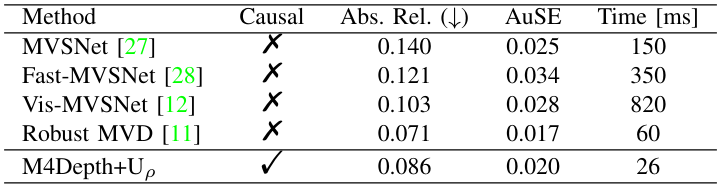
\includegraphics[width=0.7\textwidth]{32.jpg}
    \label{fig:m4d-comparison}
\end{table}

\subsection{IndoorDepth}
IndoorDepth \cite{fan2023deeper} to model głębokiej sieci neuronowej zaprojektowany do estymacji głębokości w scenach wewnętrznych. Podobnie jak GCNDepth, IndoorDepth wykorzystuje uczenie samonadzorowane, co eliminuje potrzebę etykietowanych danych głębokościowych, wykorzystując sekwencje obrazów jako sygnał nadzoru. Architektura modelu (rys. \ref{fig:indoordepth-architecture}) to splotowa sieć neuronowa z enkoderem i dekoderem, używanymi do estymacji pozycji kamery i głębokości oraz ulepszonej funkcji SSIM (od ang. structural similarity), która lepiej radzi sobie z regionami o niskiej teksturze.
\begin{figure}[H]
    \centering
    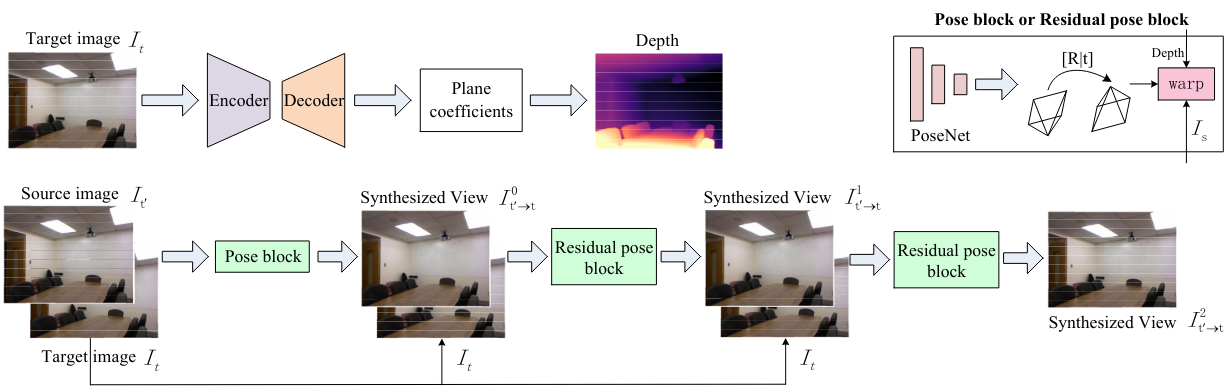
\includegraphics[width=1\textwidth]{33.jpg}
    \caption{Schemat architektury modelu IndoorDepth. Źródło: \cite{fan2023deeper}}
    \label{fig:indoordepth-architecture}
\end{figure}
Do trenowania modelu użyto zestawu danych NYUv2, składającego się z 47 tysięcy obrazów, wybranych na podstawie próbkowania co 5 klatek z surowego zestawu danych. Do testowania modelu wykorzystano oficjalny zestaw 654 obrazów z danymi o głębi z NYUv2 oraz dodatkowy zestaw ScanNet, użyty do oceny zdolności generalizacji modelu na nowych scenach wewnętrznych. Wyniki testów prezentuje tabela \ref{fig:indoordepth-results}.
\begin{table}[H]
    \centering
    \caption{Porównanie wyników działania metod nauczonych na zbiorze NYUv2. Testy wykonane zostały na zestawie ScanNet. Źródło: \cite{fan2023deeper}}
    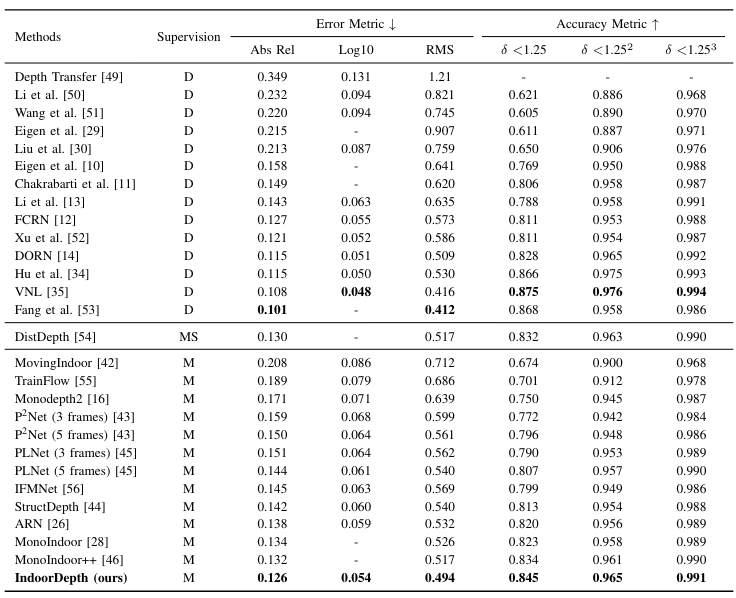
\includegraphics[width=0.9\textwidth]{34.jpg}
    \label{fig:indoordepth-results}
\end{table}

\subsection{SQLdepth}
Model SQLdepth \cite{wang2023sqldepth} jest głęboką siecią neuronową zaprojektowaną do estymacji głębokości obrazu w sposób samonadzorowany. Model SQLdepth operuje na scenach zewnętrznych, wykorzystując zestaw danych KITTI zawierający sekwencje stereo obrazów. Architektura modelu (rys. \ref{fig:sqldepth-architecture}) opiera się na splotowej sieci neuronowej z enkoderem-dekoderem, wspieranej warstwą Self Query Layer (SQL), która poprawia dokładność przewidywania głębokości.
\begin{figure}[H]
    \centering
    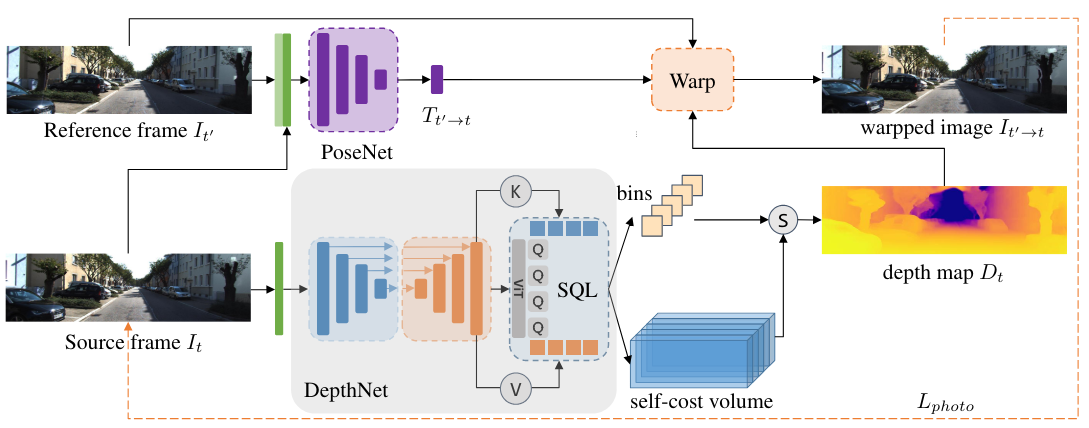
\includegraphics[width=0.9\textwidth]{35.jpg}
    \caption{Schemat architektury modelu SQLdepth. Źródło: \cite{wang2023sqldepth}}
    \label{fig:sqldepth-architecture}
\end{figure}
Podczas treningu model wykorzystuje pary stereo jako główne źródło nadzoru. Do uczenia modelu użyto około 26 tysięcy obrazów z zestawu KITTI, natomiast do testowania wykorzystano 697 obrazów z tego samego zestawu. Model był również ewaluowany na zestawach danych Cityscapes, obejmujących liczne ruchome obiekty oraz Make3D, który został użyty do oceny zdolności generalizacji modelu na wcześniej niewidzianych obrazach. Porównanie wyników metody IndoorDepth na zbiorze KITTI umieszczono w tabeli \ref{fig:sqldepth-results}.
\begin{table}[H]
    \centering
    \caption{Porównanie wyników działania metody IndoorDepth na zbiorze KITTI. Źródło: \cite{wang2023sqldepth}}
    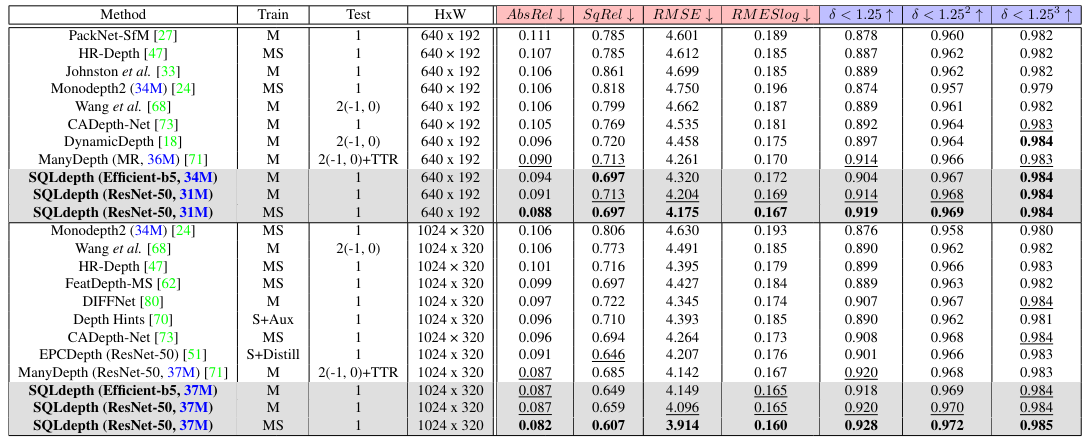
\includegraphics[width=0.95\textwidth]{36.jpg}
    \label{fig:sqldepth-results}
\end{table}


\subsection{Podsumowanie}
Przedstawione algorytmy można skategoryzować ze względu na rodzaj architektury, charakterystykę zestawów uczących i charakterystykę wyników. Poniższa tabela zawiera krótkie podsumowanie.
\begin{table}[H]
    \centering
    \caption{Podsumowanie przedstawionych modeli percepcji głębi.}
    \vspace{0.1cm}
    \resizebox{\textwidth}{!}{%
        \begin{tabular}{ |l|p{2cm}|p{2cm}|p{5cm}|p{5cm}|r| }
        \hline
        Nazwa & Architektura & Sposób uczenia & Zestawy uczące & Zestawy do oceny \\
        \hline \hline
        AdelaiDepth \cite{dosovitskiy2020} &
        rekurencyjna sieć neuronowa &
        nadzorowane &
        \begin{itemize} 
            \item Taskonomy,
            \item 3D Ken Burns, 
            \item DIML, 
            \item Holopix50K, 
            \item HRWSI. 
        \end{itemize} &
        \begin{itemize} 
            \item NYU depth V2,
            \item KITTI,
            \item ScanNet,
            \item DIODE,
            \item ETH3D,
            \item Sintel,
            \item OASIS,
            \item YouTube3D,
            \item RedWeb,
            \item iBims-1. 
        \end{itemize}\\
        \hline
        MetaPrompt-SD \cite{wan2023} &
        splotowa sieć neuronowa &
        nadzorowane &
        \begin{itemize} 
            \item NYU depth V2,
            \item KITTI.
        \end{itemize} & 
        Zestawy tożsame z uczącymi.\\
        \hline
        EVP \cite{lavreniuk2023} &
        splotowa sieć neuronowa &
        nadzorowane &
        \begin{itemize} 
            \item NYU depth V2,
            \item KITTI.
        \end{itemize} & 
        Zestawy tożsame z uczącymi.\\
        \hline
        ZoeDepth \cite{bhat2023} &
        splotowa sieć neuronowa &
        nadzorowane i częściowo nadzorowane &
        \begin{itemize} 
            \item NYU depth V2,
            \item KITTI,
            \item HRWSI,
            \item BlendedMVS,
            \item ReDWeb,
            \item DIML-Indoor,
            \item 3D Movies,
            \item MegaDepth,
            \item WSVD,
            \item TartanAir,
            \item ApolloScape,
            \item IRS.
        \end{itemize} & 
        \begin{itemize} 
            \item SUN RGB-D,
            \item iBims,
            \item DIODE,
            \item HyperSim,
            \item DDAD,
            \item DIML,
            \item Virtual KITTI 2.
        \end{itemize}\\
        \hline
        UniDepth \cite{piccinelli2024} &
        W zależności od konfiguracji splotowa sieć neuronowa lub transformator. &
        nadzorowane &
        \begin{itemize}
        \item Argoverse2,
        \item Waymo,
        \item DrivingStereo,
        \item Cityscapes,
        \item BDD100K,
        \item MapillaryPSD,
        \item A2D2,
        \item ScanNet,
        \item Taskonomy.
        \end{itemize} & 
        \begin{itemize} 
            \item SUN-RGBD,
            \item Diode Indoor,
            \item IBims-1,
            \item VOID,
            \item HAMMER,
            \item ETH-3D,
            \item nuScenes,
            \item DDAD,
            \item NYU-Depth V2,
            \item KITTI.
        \end{itemize}\\
        \hline
        \end{tabular}%
    }
    \label{tabela_podsumowanie_algorytmy}
\end{table}

\begin{table}[H]
    \centering
    \vspace{0.1cm}
    \resizebox{\textwidth}{!}{%
        \begin{tabular}{ |l|p{2cm}|p{3cm}|p{5cm}|p{5cm}|r| }
        \hline
        Depth Anything V2 \cite{yang2024depth} &
        transormator &
        częściowo nadzorowane &
        \begin{itemize}
        \item zbiory oznaczone
            \begin{itemize}
                \item BlendedMVS,
                \item Hypersim,
                \item IRS,
                \item TartanAir,
                \item VKITTI 2.
            \end{itemize}
        \item zbiory nieoznaczone
            \begin{itemize}
                \item BDD100K,
                \item Google Landmarks,
                \item ImageNet-21K,
                \item LSUN,
                \item Objects365,
                \item Open Images V7,
                \item Places365,
                \item SA-1B.
            \end{itemize}
        \end{itemize} & 
        \begin{itemize} 
            \item zbiory do oceny predykcji głębi relatywnej
            \begin{itemize} 
                \item NYU depth V2,
                \item KITTI,
                \item Sintel,
                \item DDAD,
                \item ETH3D,
                \item DIODE,
            \end{itemize}
            \item zbiory do oceny predykcji głębi metrycznej
            \begin{itemize} 
                \item SUN RGB-D,
                \item iBims-1,
                \item HyperSim,
                \item Virtual KITTI 2,
                \item DIODE Outdoor.
            \end{itemize}
        \end{itemize}\\
        \hline
        Metric3D V2 \cite{hu2024} &
        W zależności od konfiguracji splotowa sieć neuronowa lub transformator. &
        nadzorowane &
        \begin{itemize}
            \item DDAD,
            \item Lyft,
            \item Driving Stereo (DS),
            \item DIML,
            \item Arogoverse2,
            \item Cityscapes,
            \item DSEC,
            \item Mapillary PSD,
            \item Pandaset,
            \item UASOL,
            \item Virtual KITTI,
            \item Waymo,
            \item Matterport3d,
            \item Taskonomy,
            \item Replica,
            \item ScanNet,
            \item HM3d,
            \item Hypersim.
        \end{itemize} & 
        \begin{itemize}
            \item NYU,
            \item KITTI,
            \item ScanNet,
            \item NuScenes (NS),
            \item ETH3D,
            \item DIODE,
            \item iBims-1.
        \end{itemize}\\
        \hline
        DistDepth \cite{wu2022practical} &
        splotowa sieć neuronowa i transformator &
        nienadzorowane &
        \begin{itemize}
            \item SimSIN,
            \item UniSIN.
        \end{itemize} & 
        \begin{itemize}
            \item VA,
            \item NYUv2,
            \item Hypersim.
        \end{itemize}\\
        \hline
        GCNDepth \cite{masoumian2021gcndepth} &
        grafowa i rekurencyjna sieć neuronowa &
        nienadzorowane &
        \begin{itemize}
            \item KITTI
        \end{itemize} & 
        \begin{itemize}
            \item KITTI,
            \item Make3D.
        \end{itemize}\\
        \hline
        M4Depth \cite{fonder2023technique} &
        splotowa sieć neuronowa &
        nadzorowane &
        \begin{itemize}
            \item Mid-Air
        \end{itemize} & 
        \begin{itemize}
            \item Mid-Air,
            \item KITTI,
            \item TartanAir.
        \end{itemize}\\
        \hline
        IndoorDepth \cite{fan2023deeper} &
        splotowa sieć neuronowa &
        nienadzorowane &
        \begin{itemize}
            \item NYUv2
        \end{itemize} & 
        \begin{itemize}
            \item NYUv2,
            \item ScanNet.
        \end{itemize}\\
        \hline
        SQLdepth \cite{wang2023sqldepth} &
        splotowa sieć neuronowa &
        nienadzorowane &
        \begin{itemize}
            \item KITTI
        \end{itemize} & 
        \begin{itemize}
            \item KITTI,
            \item Cityscapes,
            \item Make3D.
        \end{itemize}\\
        \hline
        \end{tabular}%
    }
    \label{tabela_podsumowanie_algorytmy_2}
\end{table}

\section{Zbiory danych}
\subsection{KITTI (Karlsruhe Institute of Technology and Toyota Technological Institute)}
Wiodącym zestawem danych używanym do trenowania i oceny algorytmów percepcji głębi jest opracowany przez niemiecki Instytut Technologii Karlsruhe'a oraz amerykański Instytut Technologii Toyota zbiór KITTI\footnote{Nazwa KITTI jest skrótem nazw instytutów, przez które zbiór został opracowany.} \cite{geiger2012}. Zawiera on 93 tysiące obrazów RGBD zarejestrowanych przy pomocy autorskiej platformy jezdnej Annieway (rys. \ref{fig:kitti-annieway-example}) składającej się z lasera firmy Velodyne \cite{Velodyne}, kamer kolorowych i monochromatycznych oraz systemu GPS zamontowanych na samochodzie osobowym. Obrazy należące do tego zbioru podzielone zostały na pięć kategorii: drogi, miasta, osiedla, kampus i osoby. Prezentują one zatem sceny zewnętrzne.
\begin{figure}[H]
    \centering
    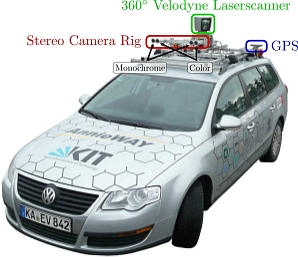
\includegraphics[width=0.4\textwidth]{23.jpg}
    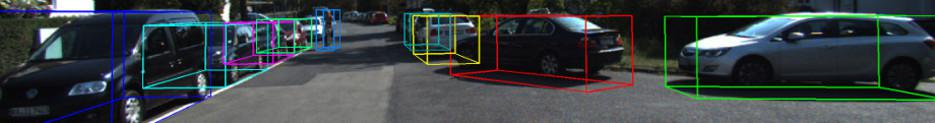
\includegraphics[width=1\textwidth]{37.jpg}
    \caption{Rejestrująca platforma jezdna użyta w przygotowaniu zbioru KITTI oraz przykładowy obraz. Źródło: \cite{geiger2012}}
    \label{fig:kitti-annieway-example}
\end{figure}

\subsection{NYUv2 (NYU-Depth V2)}
Drugim najczęściej wykorzystywanym zestawem obrazów jest NYUv2 przedstawiony w 2012 r. w \cite{couprie2013}. Zestaw ten składa się z 407024 obrazów RGB z odpowiadającymi im mapami głębi przygotowanymi przy użyciu urządzenia Microsoft Kinect. Autorzy skategoryzowali obrazy w zbiorze na następujące kategorie: piwnice, łazienki, sypialnie, księgarnia, kawiarnia, salony, jadalnie, sklepy meblowe, biura, kuchnie, biblioteki, bawialnie i inne. Obrazy przygotowane przez autorów NYUv2 przedstawiają wyłącznie sceny wewnątrz budynków. Niniejszy zestaw jest również wykorzystywany w dziedzinie segmentacji obrazu ze względu na przygotowane oznaczenie obrazów. Przykładową scenę z mapą głębi i segmentacją umieszczono na rys. \ref{fig:nyuv2-example}.
\begin{figure}[H]
    \centering
    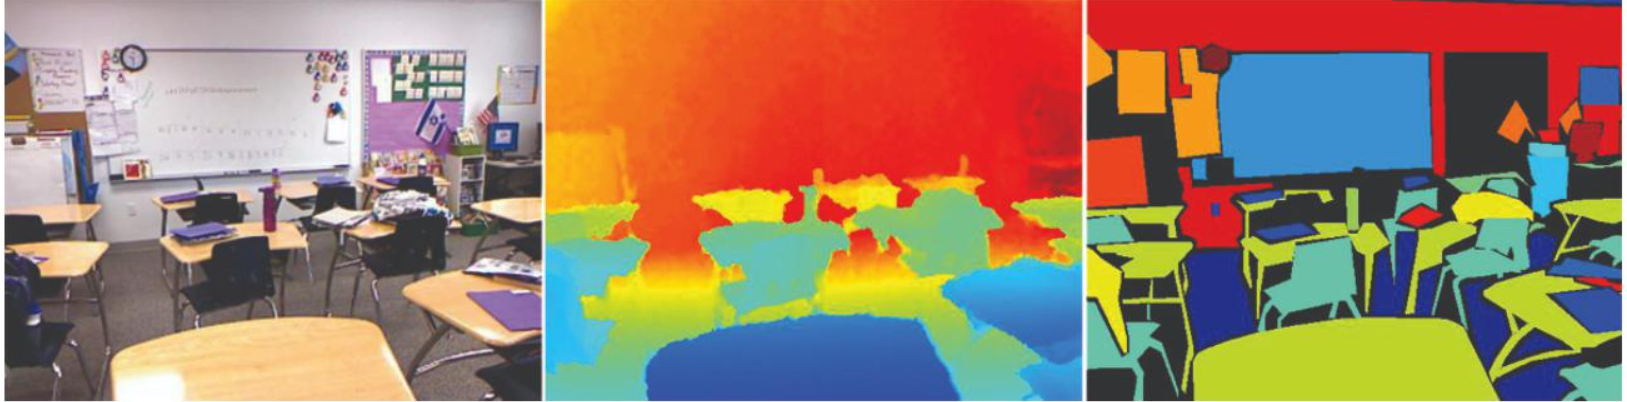
\includegraphics[width=0.65\textwidth]{38.jpg}
    \caption{Przykładowy obraz z zestawu NYUv2 ze zmierzoną głębią i segmentacją. Źródło: \cite{couprie2013}}
    \label{fig:nyuv2-example}
\end{figure}

\subsection{DIODE (Dense Indoor and Outdoor Depth)}
Zbiór DIODE \cite{vasiljevic2019} jest wyjątkowy na tle konkurencji przez wzgląd na różnorodność scen. Jest bowiem pierwszym publicznie dostępnym zestawem obrazów prezentujących sceny zewnętrzne i wewnętrzne. Większa różnorodność scen pozwala na uzyskanie lepszych wyników na płaszczyźnie generalizacji modeli percepcji głębi. Na ten zbiór składa się 8574 obrazów scen wewnętrznych oraz 16884 obrazy scen zewnętrznych zarejestrowanych za pomocą tego samego urządzenia - skanera FARO Focus S350. Rysunek \ref{fig:diode-example} zawiera przykładowe sceny z zestawu. Przygotowane przez twórców zbioru porównanie z podobnymi zestawami (rys. \ref{fig:diode-comparison}) wskazuje na wysoką dokładność i zasięg zastosowanej aparatury.
\begin{figure}[H]
    \centering
    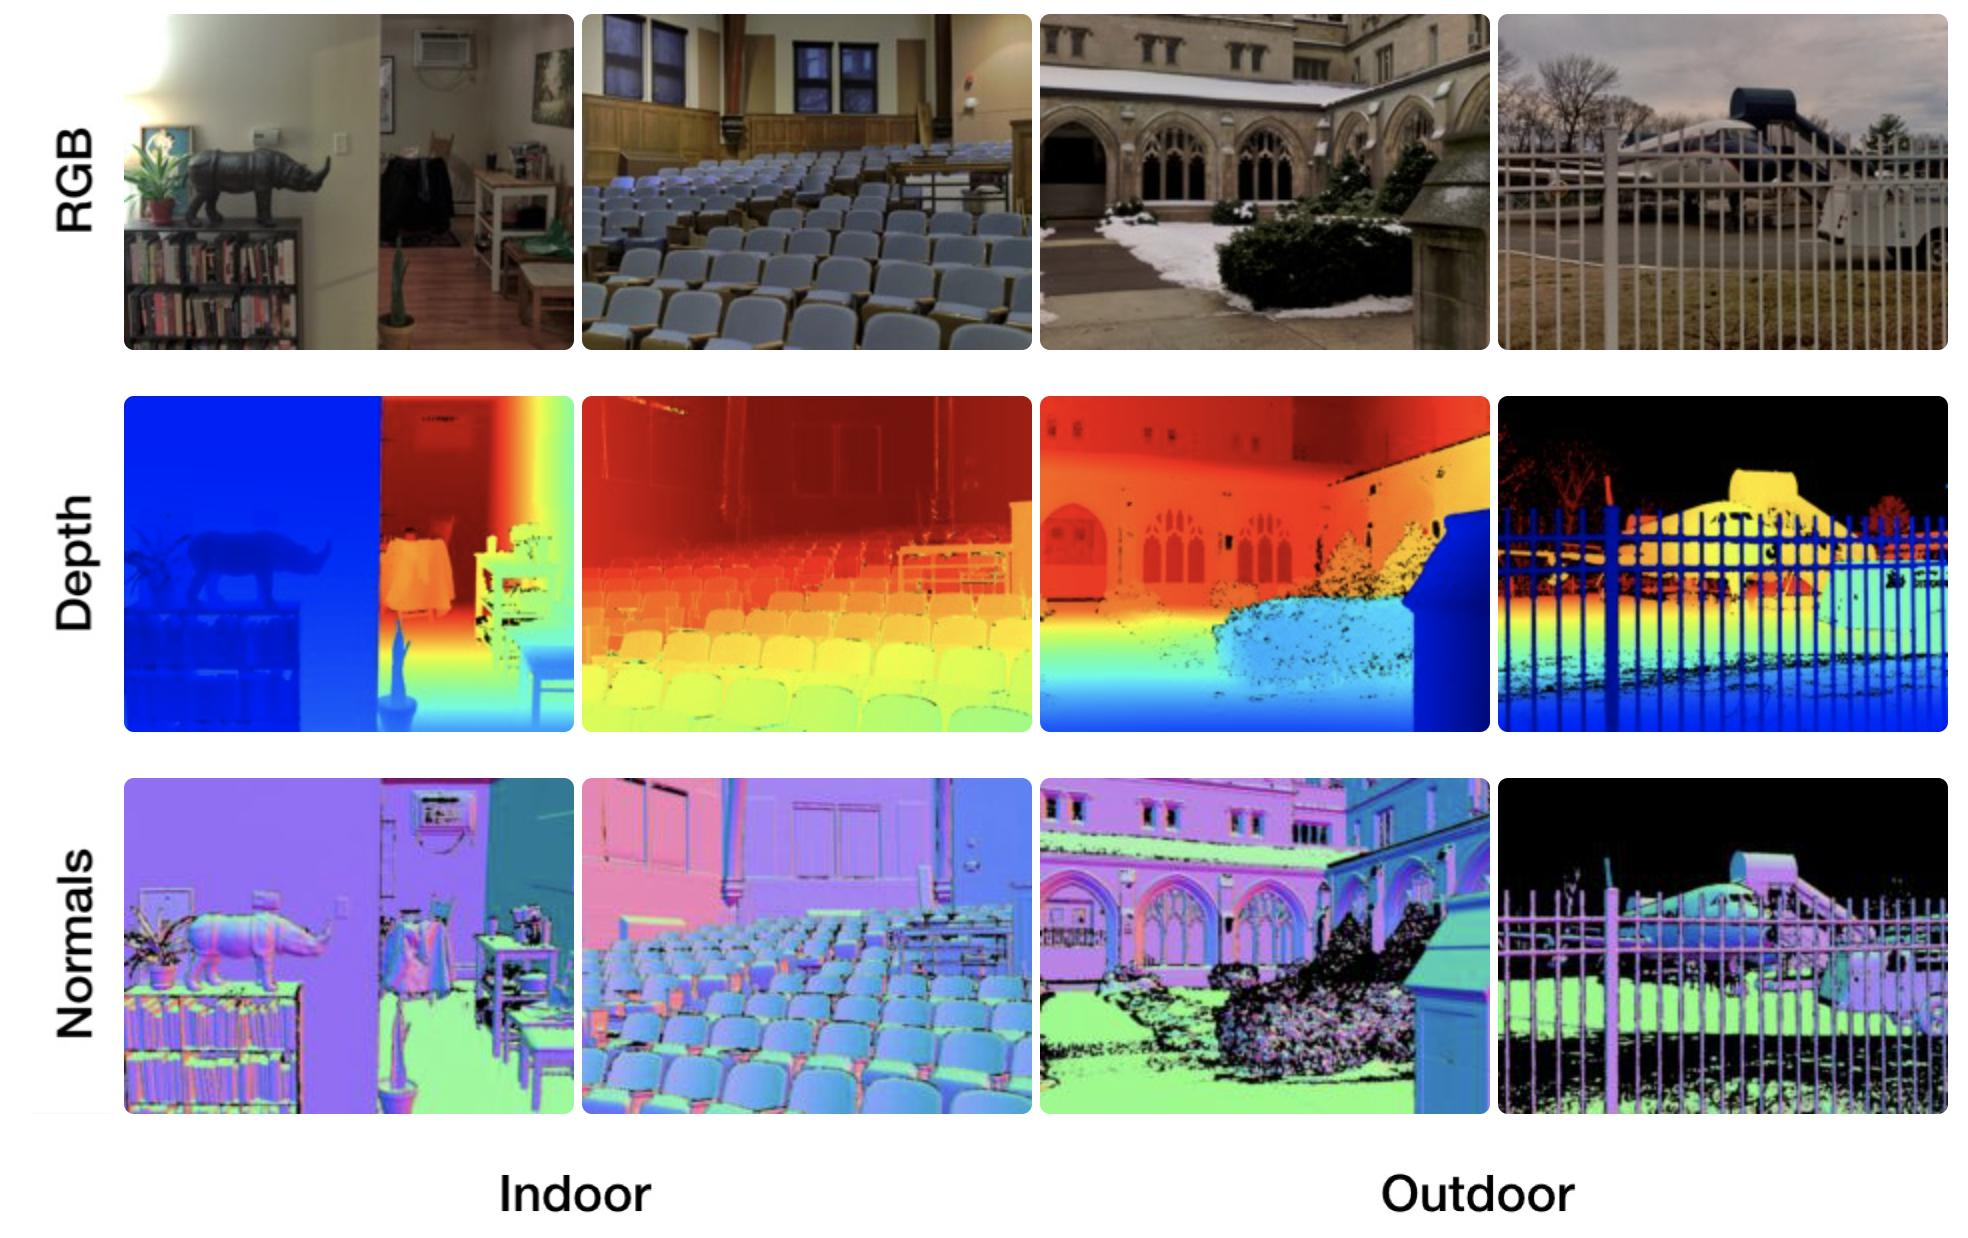
\includegraphics[width=0.65\textwidth]{39.jpg}
    \caption{Przykładowe obrazy z głębią i normalnymi powierzchni. Źródło: \cite{vasiljevic2019}}
    \label{fig:diode-example}
\end{figure}
\begin{table}[H]
    \centering
    \caption{Porównanie statystyk zbioru DIODE z innymi popularnymi zbiorami danych. Źródło: \cite{vasiljevic2019}}
    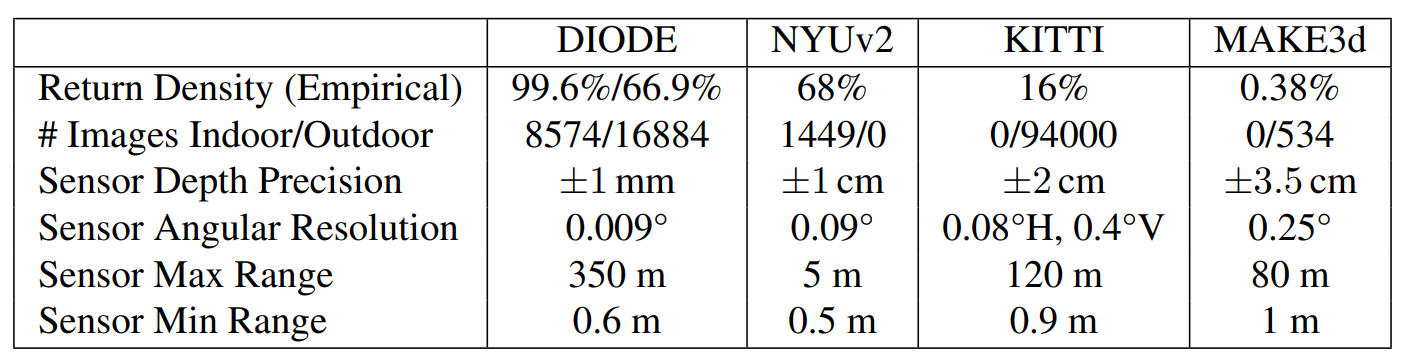
\includegraphics[width=0.65\textwidth]{24.jpg}
    \label{fig:diode-comparison}
\end{table}

\subsection{SUN RGB-D}
Głównym założeniem zestawu SUN RGB-D \cite{song2015} jest dostarczenie danych dla modeli interpretujących trójwymiarowe sceny. Składa się on z 10335 obrazów pomieszczeń wewnętrznych z mapami głębi pochodzącymi z sensorów Intel Realsense, Asus Xtion i obu wersji Microsoft Kinect. Na rzeczone obrazy zostały naniesione trójwymiarowe oznaczenia widniejących przedmiotów. Z powodu odmiennego przeznaczenia, zbiór ten jest często wykorzystywany w celu oceny efektywności modeli percepcji głębi. Przykładowe sceny oraz urządzenia rejestrujące przedstawione zostały na rysunku \ref{fig:sunrgbd-comparison}.
\begin{figure}[H]
    \centering
    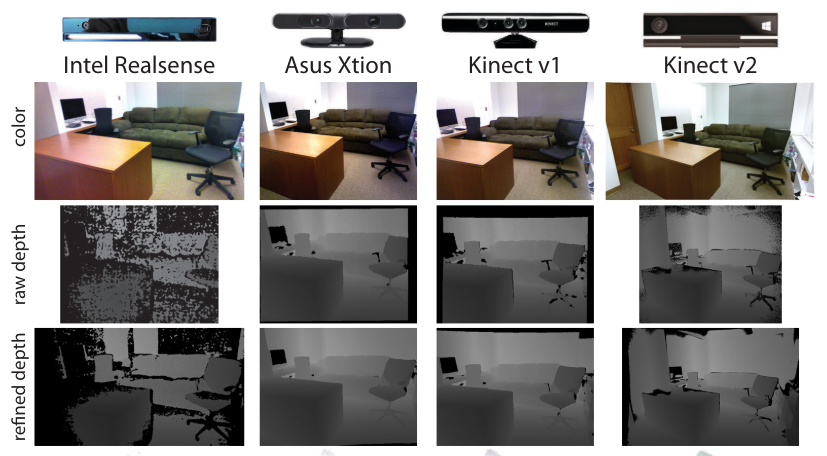
\includegraphics[width=0.75\textwidth]{40.jpg}
    \caption{Przykładowe obrazy ze zbioru z głębią zarejestrowaną i poprawioną za pomocą krótkich nagrań wideo. Źródło: \cite{song2015}}
    \label{fig:sunrgbd-comparison}
\end{figure}

\subsection{Matterport3D}
W 2017 r. firma Matterport zaprezentowała zestaw danych nazwany Matterport3D \cite{chang2017} przygotowany przy pomocy autorskiego urządzenia rejestrującego. Zestaw składa się z 10800 zdjęć panoramicznych złożonych z 194400 obrazów z odpowiadającą im mapą głębi. Zdjęcia w zbiorze przedstawiają 90 scen przedstawiających wnętrza budynków. Obrazy i modele wchodzące w skład zbioru przedstawia rysunek \ref{fig:matterport3d-example}.
\begin{figure}[H]
    \centering
    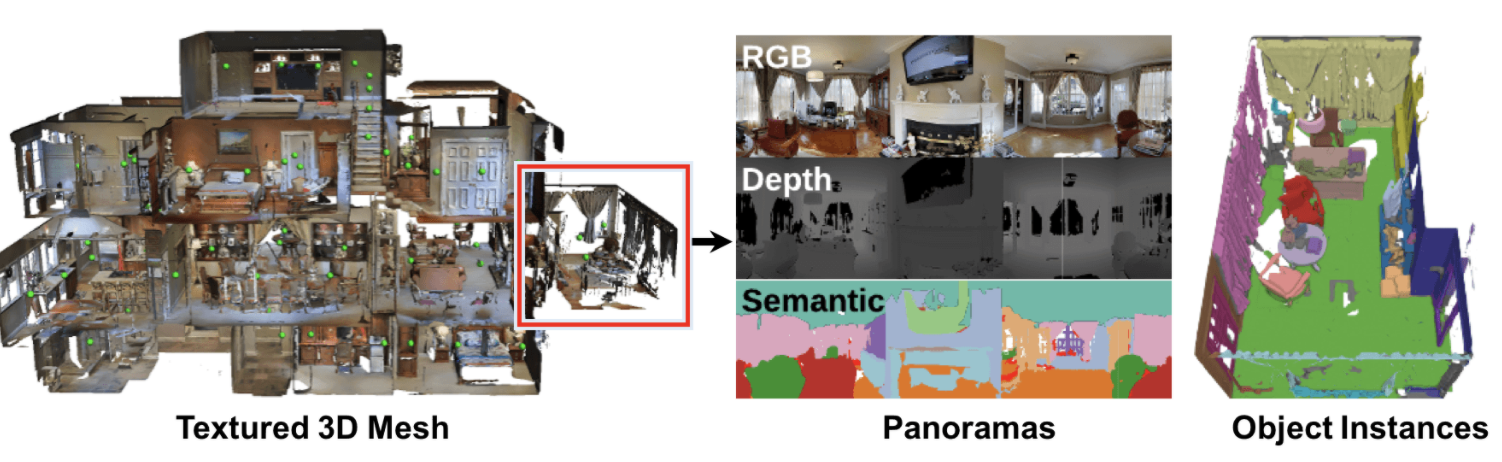
\includegraphics[width=0.9\textwidth]{41.jpg}
    \caption{Przykładowe obrazy i modele ze zbioru z głębią zarejestrowaną i segmentacją. Źródło: \cite{chang2017}}
    \label{fig:matterport3d-example}
\end{figure} 

\subsection{DDAD (Dense Depth for Autonomous Driving)}
Zestaw DDAD \cite{guizilini2020} został stworzony przez Toyota Research Institute. Zawiera 17050 obrazów treningowych i 4150 obrazów do oceny modelu, w tym zróżnicowane próbki scen miejskich i autostradowych z całego świata nagrane przez flotę samochodów autonomicznych wyposażonych w kamery i lasery LIDAR Luminar-H2. Wykorzystywany jest głównie do ewaluacji i rozwijania metod estymacji głębi w prowadzeniu pojazdów. Zestaw DDAD został wykorzystany do przetrenowania modelu PackNet tego samego autorstwa, nie osiąga on jednak wyników porównywalnych do wybranych w niniejszej pracy modeli.
Rysunek \ref{fig:ddad-example} to przykładowa scena z tego zestawu.
\begin{figure}[H]
    \centering
    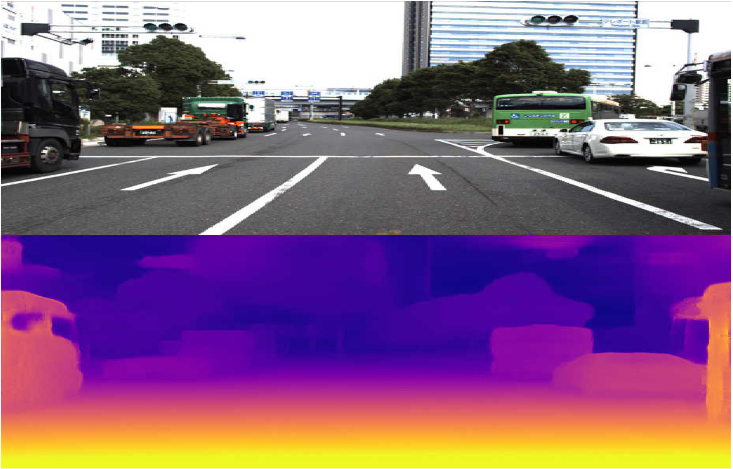
\includegraphics[width=0.35\textwidth]{42.jpg}
    \caption{Przykładowy obraz i mapa głębi z zestawu DDAD. Źródło: \cite{guizilini2020}}
    \label{fig:ddad-example}
\end{figure} 

\subsection{SYNS-Patches}
Zestaw SYNS-Patches \cite{spencer2022deconstructing} jest rozszerzeniem zestawu zaprezentowanego w 2016 r. w \cite{adams2016syns}. W stosunku do oryginału, który zawierał 92 sceny w 9 różnych kategoriach został urozmaicone o odmiennie scharakteryzowane sceny, w tym między innymi lasy, tereny przemysłowe oraz wnętrza budynków. Zbiór SYNS-Patches dostarcza bardzo wysokiej jakości skany LIDAR również scen zewnętrznych, które według twórców w podobnych rozwiązaniach są znacznie rzadziej etykietowane\footnote{Zestaw SYNS-Patches posiada aż 78,30\% pokrycie obrazu mapą głębi, podczas gdy zestaw KITTI posiada jedynie 15,28\% pokrycie.}. Na finalny zbiór składa się 1175 obrazów panoramicznych i zarejestrowanych w technologii HDR za pomocą urządzenia Spheron SpheroCam HDR oraz skanera LIDAR Leica ScanStation P20. Istotną kwestią w kontekście tego zestawu jest fakt, że mapy głębi nie zostały publicznie udostępnione ze względu na jego przeznaczenie wyłącznie do oceny działania modeli. Autorzy chcą w ten sposób uniknąć dopasowania do przedstawionych w zbiorze scen w procesie uczenia. Przykłady obrazów z zestawu SYNS-Patches ujęte zostały na rysunku \ref{fig:syns-example}.
\begin{figure}[H]
    \centering
    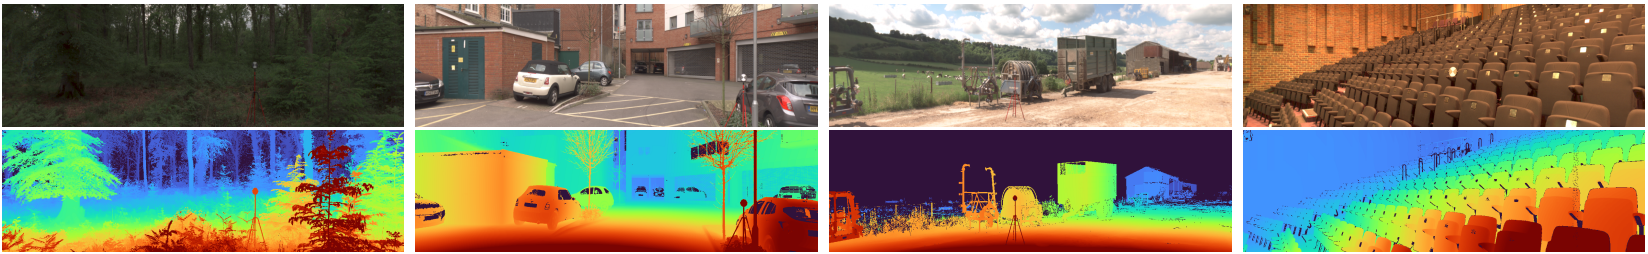
\includegraphics[width=1\textwidth]{44.jpg}
    \caption{Przykłady obrazów z zestawu SYNS-Patches z odpowiadającymi im mapami głębi. Źródło: \cite{spencer2022deconstructing}}
    \label{fig:syns-example}
\end{figure}

\subsection{Cityscapes}
Cityscapes \cite{cordts2016cityscapes} to zestaw danych skompletowany w 2016 r. którego głównym założeniem jest wykorzystanie w środowiskach aplikacyjnych, gdzie kluczową kwestię stanowi zrozumienie scen miejskich. Jest to powodem skupienia autorów na aspekcie segmentacji obrazów. Mimo to, zestaw Cityscapes jest często wykorzystywany w kontekście algorytmów percepcji głębi ze względu na zawartość mapy głębi do każdej sceny w nim zawartej. Zbiór ten składa się z 5 tysięcy obrazów etykietowanych z bardzo wysoką dokładnością do jednego piksela oraz 20 tysięcy obrazów etykietowanych ze znacznie zmniejszoną dokładnością dla algorytmów, które potrafią czerpać korzyść z większej ilości danych w procesie uczenia. Przykłady obrazów z obu podzbiorów przedstawia rysunek \ref{fig:cityscapes-example}. Obrazy przedstawiają sceny miejskie rejestrowane w świetle dziennym z 50 różnych miast w Niemczech. Zostały zarejestrowane przy pomocy kamer stereo zamontowanych na pojeździe.
\begin{figure}[H]
    \centering
    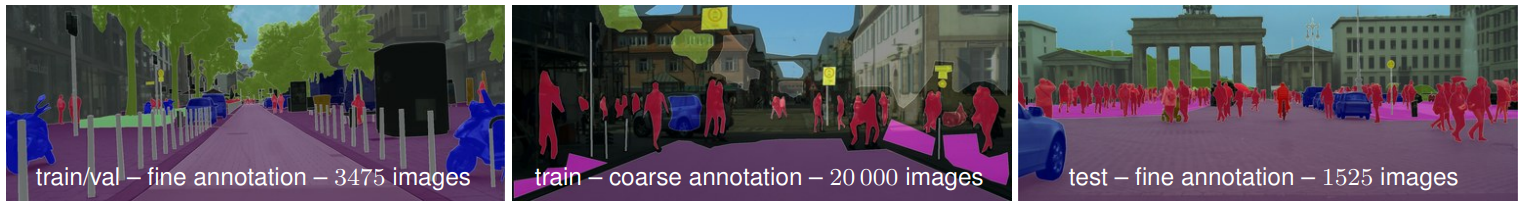
\includegraphics[width=0.9\textwidth]{43.jpg}
    \caption{Przykłady obrazów z zestawu Cityscapes. Źródło: \cite{cordts2016cityscapes}}
    \label{fig:cityscapes-example}
\end{figure}

\subsection{Virtual KITTI 2}
Virtual KITTI 2 \cite{cabon2020virtualkitti2} jest ulepszonym względem pierwszej wersji zestawem syntetycznych obrazów wygenerowanych komputerowo na wzór przedstawionych w zestawie KITTI \cite{geiger2012} scen ruchu ulicznego. Ulepszenie polegało na powiększeniu zakresu danych w zbiorze - poza mapami głębi dodano między innymi segmentację obiektów - oraz na podwyższeniu rozdzielczości obrazów.

Wirtualny odpowiednik jednego z najpowszechniejszych zbiorów danych powstał ze względu na szeroki wachlarz możliwości manipulacji charakterystyką scen za pomocą oprogramowania. Zestaw ten zawiera bowiem identyczną sekwencję obrazów jednak w różnych warunkach pogodowych oraz różnych konfiguracjach wirtualnej kamery. Ze względu na syntetyczny charakter zbioru zawiera on bardzo dokładne informacje o głębi, ponieważ wygenerowane dane nie są obarczone błędem pomiarowym.
Rysunek \ref{fig:vkitti-example} prezentuje przykładową scenę z zestawu Virtual KITTI 2.
\begin{figure}[H]
    \centering
    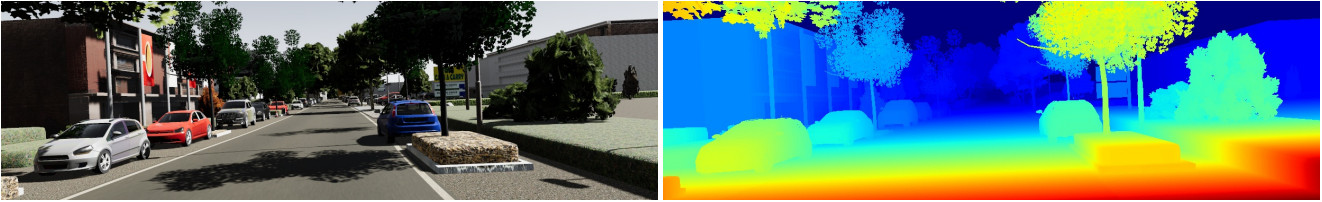
\includegraphics[width=1\textwidth]{47.jpg}
    \caption{Przykładowa scena z zestawu Virtual KITTI 2. Źródło: \cite{cabon2020virtualkitti2}}
    \label{fig:vkitti-example}
\end{figure}

\subsection{Taskonomy}
Zestaw Taskonomy \cite{zamir2018taskonomydisentanglingtasktransfer} zawiera cztery miliony komputerowo wygenerowanych obrazów oznaczonych za pomocą danych z dwudziestu sześciu różnych dziedzin widzenia komputerowego. Poza mapami głębi zestaw zawiera również dane dotyczące normalnych powierzchni, krawędzi obiektów czy segmentacji semantycznej. Tak bogate oznaczenia powodują, że rozwiązanie to jest często wykorzystywane jako główny zestaw uczący wielu modeli z kategorii widzenia komputerowego. Podobnie jak w przypadku Virtual KITTI 2 oznaczenia są maksymalnie dokładne ze względu na brak ograniczeń sprzętowych i pozostałych uwarunkowań wynikających z fizycznej rejestracji danych. Jeden z obrazów ze zbioru Taskonomy został przedstawiony na rysunku \ref{fig:taskonomy-example}.

\begin{figure}[H]
    \centering
    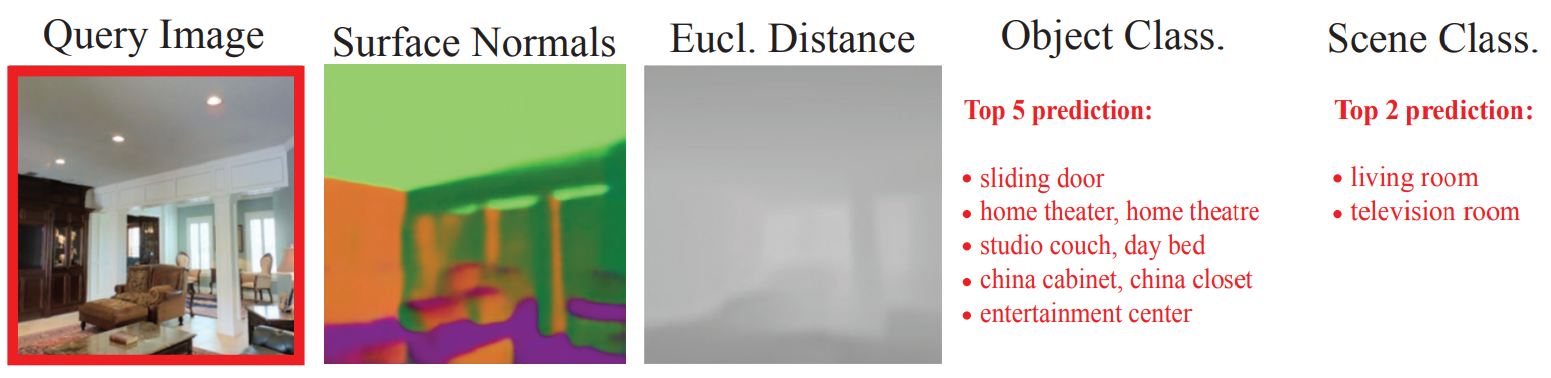
\includegraphics[width=0.65\textwidth]{48.jpg}
    \caption{Przykładowy obraz z zestawu Taskonomy wraz z oznaczeniami z różnych kategorii. Źródło: \cite{zamir2018taskonomydisentanglingtasktransfer}}
    \label{fig:taskonomy-example}
\end{figure}

\subsection{Podsumowanie}
Przedstawione w niniejszym rozdziale zestawy danych przyczyniły się w znacznej mierze do rozwoju metod predykcji głębi. Rozbieżność ich cech z kolei przyczynia się pozytywnie do generalizacji modeli. Poniższa tabela stanowi wykaz przedstawionych zestawów z podziałem na najważniejsze kategorie.
\begin{table}[H]
    \centering
    \caption{Podsumowanie przedstawionych zbiorów danych używanych przez algorytmy percepcji głębi.}
    \vspace{0.1cm}
    \resizebox{\textwidth}{!}{%
        \begin{tabular}{ |p{3cm}|p{3cm}|p{5cm}|p{5cm}|r| }
        \hline
        Nazwa & Charakterystyka obrazów & Liczebność zbioru & Urządzenie rejestrujące głębię \\
        \hline \hline
        KITTI \cite{geiger2012} &
        sceny zewnętrzne & 
        93 000 &
        Skaner laserowy Velodyne \cite{Velodyne} i system lokalizacji GPS. \\
        \hline
        NYUv2 \cite{couprie2013} &
        sceny wewnętrzne & 
        407 024 &
        Microsoft Kinect \\
        \hline
        DIODE \cite{vasiljevic2019} &
        sceny zewnętrzne i wewnętrzne & 
        25 458 &
        Skaner FARO Focus S350 \\
        \hline
        SUN RGB-D \cite{song2015} &
        sceny wewnętrzne & 
        10 335 &
        Intel RealSense 3D, Asus Xtion LIVE PRO i Microsoft
Kinect. \\
        \hline
        Matterport3D \cite{chang2017} &
        sceny wewnętrzne & 
        194 400 &
        autorska konstrukcja Matterport  \\
        \hline
        DDAD \cite{guizilini2020} &
        sceny zewnętrzne & 
        21 200 &
        Luminar-H2  \\
        \hline
        SYNS-Patches \cite{adams2016syns} &
        sceny zewnętrzne i wewnętrzne & 
        1 175 &
        Leica ScanStation P20  \\
        \hline
        Cityscapes \cite{cordts2016cityscapes} &
        sceny zewnętrzne & 
        25 000 &
        autorska konsktrukcja kamer stereo na pojeździe
        \\
        \hline
        Virtual KITTI 2 \cite{cabon2020virtualkitti2} &
        sceny zewnętrzne & 
        63 730 &
        syntetyczne obrazy wygenerowane komputerowo
        \\
        \hline
        Taskonomy \cite{zamir2018taskonomydisentanglingtasktransfer} &
        sceny wewnętrzne & 
        4 000 000 &
        syntetyczne obrazy wygenerowane komputerowo
        \\
        \hline
        \end{tabular}%
    }
    \label{tabela_podsumowanie_zbiory}
\end{table}